\documentclass{article}

\usepackage{NotesPackage}

\usepackage[version=4]{mhchem}
\usepackage{caption}
\captionsetup{justification=centering}

\newcommand{\notesVersion}{1.0}
\newcommand{\notesDate}{04/01/2021}

\author{Willoughby Seago}
\date{14 January, 2020}
\title{Physics of Matter}
\begin{document}
    \maketitle
    These are my notes for the \textit{matter} part of the \textit{physics of fields and matter} course from the University of Edinburgh as part of the second year of the theoretical physics degree.
    When I took this course in the 2019/20 academic year it was taught by Dr Stewart McWilliams\footnote{\url{https://www.ph.ed.ac.uk/people/stewart-mcwilliams}} and Dr Simon Titmuss\footnote{\url{https://www.ph.ed.ac.uk/people/simon-titmuss}}.
    These notes are based on the lectures delivered as part of this course, and the notes provided as part of this course.
    The content within is correct to the best of my knowledge but if you find a mistake or just disagree with something or think it could be improved please let me know.
    
    These notes were produced using \LaTeX\footnote{\url{https://www.latex-project.org/}}.
    Graphs where plotted using Python\footnote{\url{https://www.python.org/}}, Matplotlib\footnote{\url{https://matplotlib.org/}}, NumPy\footnote{\url{https://numpy.org/}}, and SciPy\footnote{\url{https://scipy.org/scipylib/}}.
    Diagrams were drawn with tikz\footnote{\url{https://www.ctan.org/pkg/pgf}}.
    Some images were taken from the lecture notes provided.
    
    This is version \notesVersion~of these notes, which is up to date as of \notesDate.
    \begin{flushright}
        Willoughby Seago
        
        s1824487@ed.ac.uk
    \end{flushright}
    \clearpage
    \tableofcontents
    \listoffigures
    \listoftables
    \clearpage
    
    \part{Fluids}
    \section{The Basics}
    \subsection{Scale}
    This course is mostly interested in large collections of particles where large is approximately \SI{1}{mol}.
    The mole is defined as the one Avogadro's number \(N_A\) of particles, that is the number of particles in \SI{12}{g} of carbon-12.
    \[N_A = \num{6.022e23}\]
    This is such a large number that considering individual particles to see macroscopic effects is a hopeless task.
    The size of molecules is measured in angstroms \si{\angstrom} where \(\SI{1}{\angstrom} = \SI{e-10}{m}\).
    
    \subsection{Brownian Motion}
    Brownian motion is the random movement of particles suspended in a fluid.
    It arises as the net effect of many molecular impacts.
    This was key evidence for the molecular nature of matter.
    
    \subsection{Random Walks}
    A random walk is a path characterised by a number of equal sized steps that are equally likely to be in any direction.
    Random walks have structure at every level.
    What this means is that if you where to take steps more frequently you would still have a random walk.
    
    We use the notation \(\expected{x}\) to represent the average value of \(x\), theoretically over an infinite number of measurements.
    If a random walk of \(N\) steps ends at \(\vv r_N\) then
    \[\expected{\vv r_N} = \vv 0\]
    This is because steps in all directions are equally likely so over many walks cancel out.
    The average distance from the origin squared is given by
    \[\expected{r_N^2} = N\lambda^2\]
    where \(\lambda\) is the step length and \(r_N^2 = \vv r_N\cdot\vv r_N\).
    This is easily shown in 1 dimension.
    \[\vv r_N = \vv r_{N-1} \pm \vv \lambda\]
    \[\expected{r_N^2} = \expected{r_{N-1}^2} + 2\expected{\vv r_{N-1}\cdot\vv \lambda} + \lambda^2\]
    Forward and backward steps are equally likely so \(\expected{\vv r_{N-1}\cdot\vv \lambda} = 0\).
    Our basis case is one step, \(N = 1\).
    After one step the distance from the origin in \(\lambda\) regardless of direction so \(r_N^2 = \lambda^2\).
    Now assume that \(\expected{r_k} = k\lambda^2\).
    Hence the distance squared after \(k+1\) steps is
    \[\expected{r_{k+1}} = \expected{r_k^2} + \lambda^2 = k\lambda^2 + \lambda^2 = (k+1)\lambda^2\]
    so by induction
    \[\expected{r_N^2} = N\lambda^2\]
    If one step is taken every \(\Delta t\) seconds then in time \(t\) \(N = t/\Delta t\) steps are taken.
    Hence \(\expected{r_N^2}\propto N \propto t\).
    This comes in useful when considering diffusion which is characterised by
    \[\expected{r_N^2} \propto Dt\]
    where \(D\) is the diffusion coefficient.
    
    If molecules are so small and the particles the hit are (relatively) big and molecules are going at (relatively) low speeds (\SIrange{100}{1000}{m/s}) then how do they impart enough of a change of momentum to be noticeable?
    Einstein realised that we don't see the effects of the rapid motion of individual impacts but that we only see the rare large displacements.
    
    \section{Maxwell--Boltzmann Distribution}
    \subsection{Equipartition}
    Einstein realised that colloidal particles behave just like solute particles but bigger.
    The equipartition theory is that energy is shared equally between all modes of a system.
    The mean energy of each quadratic mode (any mode with dependence on something squared) is \(\frac{1}{2}k_BT\) where \(k_B\) is the Boltzmann constant \(k_B = \SI{1.38e-23}{J.K^{-1}}\) and \(T\) is the temperature in kelvin.
    For example if each particle has kinetic energy \(E_K\) then
    \[\expected{E_K} = \frac{1}{2}mv^2 = \frac{1}{2}m\left(\expected{v_x^2} + \expected{v_y^2} + \expected{v_z^2}\right) = \frac{3}{2}k_BT\]
    We can be precise about average molecular energies but not individual particles.
    
    \subsection{Probability Recap}
    If we measure some property \(x\) \(N\) times and we find \(x_i\) \(N_i\) times then the mean is
    \[\expected{x} = \sum_i\frac{N_i}{N}x_i = \sum_i P_ix_i\]
    where \(P_i = N_i/N\) is the probability of \(x_i\).
    This is for a discrete distribution.
    We can extend it to a continuous distribution by using an integral over all possible values of \(x\) and a probability distribution function \(P\) in place of \(P_i\):
    \[\expected{x} = \int_{-\infty}^{\infty}xP(x)\,dx\]
    When we are talking about molecule's speeds the probability distribution we use is the Maxwell--Boltzmann distribution \(f\).
    
    \subsection{Maxwell--Boltzmann Distribution}\label{sec:boltzmann factor}
    Let \(g(v_x)dv_x\) be the fraction of particles with velocities \(v_x\to v_x + dv_x\).
    The velocity distribution function \(g\) is proportional to the Boltzmann constant.
    The Boltzmann constant in general is proportional to the probability \(P\) that a system is in a state with energy \(E\).
    \[P\propto e^{-E/k_BT}\]
    where \(E\) is the energy in question.
    In the case of particle speeds \(E\) is the kinetic energy so
    \[g(v_x) \propto \exp\left(-\frac{mv_x^2}{2k_BT}\right)\]
    We need to normalise the distribution:
    \[\int_{-\infty}^{\infty} g(v_x)dv_x = 1\]
    \[\int_{-\infty}^{\infty} \exp\left(-\frac{mv_x^2}{2k_BT}\right) = \sqrt{\frac{2\pi k_BT}{m}}\]
    \[g(v_x) = \sqrt{\frac{m}{2\pi k_BT}}\exp\left(-\frac{mv_x^2}{2k_BT}\right)\]
    The fraction with velocities \(v_x\to v_x + dv_x\), \(v_y\to v_y + dv_y\), \(v_z\to v_z + dv_z\) is given by
    \[g(v_x)dv_xg(v_y)dv_yg(v_z)dv_z = \left(\frac{m}{2\pi k_BT}\right)^{3/2}\exp\left(-\frac{mv^2}{2k_BT}\right)dv_xdv_ydv_z\]
    Since all directions are equally likely the situation in velocity space is spherically symmetric.
    The volume of velocity space corresponding to speeds \(v\to v + dv\) is a spherical shell with inner radius \(v\) and outer radius \(v + dv\).
    The volume of this shell is \(4\pi v^2dv\).
    As \(v\) increases there are more ways to combine \(v_x\), \(v_y\) and \(v_z\) to get \(v\) hence as \(v\) increases so does the volume.
    The fraction of particles with speeds \(v\to v + dv\) is
    \[f(v)dv = 4\pi v^2g(v_x)g(v_y)g(v_z)dv\]
    \[f(v)dv = \frac{4}{\sqrt{\pi}}\left(\frac{m}{2k_BT}^{3/2}\right)v^2\exp\left(-\frac{mv^2}{2k_BT}\right)\]
    \begin{figure}[ht]
        \centering
        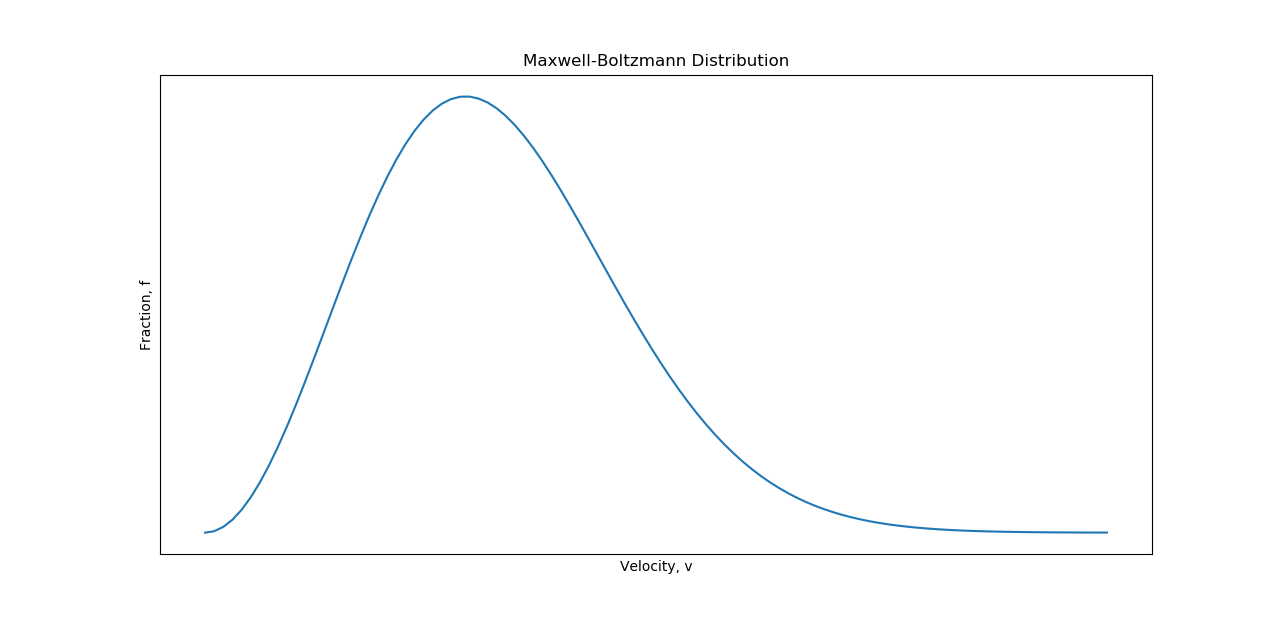
\includegraphics[scale=0.5]{Maxwell_Boltzmann_distribution.png}
        \caption{The Maxwell--Boltzmann distribution}
    \end{figure}
    The most probable speed \(v^*\) is found by requiring \(f(v^*)\) to be a maximum:
    \[\pdvat{f}{v}{v^*} = 0\]
    \[\pdv{f}{v} = \frac{4}{\sqrt{\pi}} \left(-\frac{m}{2k_BT}\right)^{3/2} \left[2v\exp\left(-\frac{mv^2}{2k_BT}\right) - \frac{mv^3}{2k_BT} \exp\left(-\frac{mv^2}{2k_BT}\right)\right] = 0\]
    The value in the square brackets must be 0.
    This gives
    \[v^* = \sqrt{\frac{2k_BT}{m}}\]
    We can also find the expected value of the velocity:
    \begin{align*}
        \expected{v} &= \int_0^\infty vf(v)\, dv\\
        &= \frac{4}{\sqrt{\pi}}\left(-\frac{m}{2k_BT}\right)^{3/2} \int_0^\infty v^3\exp\left(-\frac{mv^2}{2k_BT}\right)\,dv\\
        &= \sqrt{\frac{8k_BT}{\pi m}}
    \end{align*}
    From this and the mean kinetic energy we can also work out the root mean square:
    \[\expected{E_K} = \frac{1}{2}m\expected{v^2} = \frac{3}{2}k_BT \implies \sqrt{\expected{v^2}} = v_\mathrm{rms} = \sqrt{\frac{3k_BT}{m}}\]
    By looking purely at the numerical factors it is clear that the most probable speed is the lowest, then the mean speed and the root mean square speed is highest (note that \(2 < 8/\pi < 3\)).
    
    \example
    What is the mean speed of \ce{N2} at \SI{300}{K}?
    
    The molar mass of \ce{N2} is \(\SI{28}{g.mol^{-1}}\).
    This means that the mass of one molecule is \(\num{28e-3}/N_A\,\si{kg}\).
    This gives \(\expected{v} = \SI{476}{m.s^{-1}}\).
    This is comparable to the speed of sound in air.
    
    We can now show that Equipartition works for kinetic energy:
    \begin{align*}
        \expected{E_K} &= \frac{1}{2}m\expected{v^2}\\
        &= \frac{1}{2}m\int_0^\infty v^2 f(v)\,dv\\
        &= \frac{1}{2}m\frac{4}{\sqrt{\pi}}\left(\frac{m}{2k)BT}\right)^{3/2} \int_0^{\infty}v^4 \exp\left(-\frac{mv^2}{2k_BT}\right) \,dv\\
        &= \frac{3}{2}k_BT
    \end{align*}
    The temperature provides a measure of mean kinetic energy which is independent of mass.
    Equipartition generally only applies at high temps where the energy levels are close enough together to approximate as continuous, how high depends on the specific energy levels.
    
    Equipartition applies to any quadratic mode, for example a mass spring system has \(\expected{E_P} = kx^2/2\).
    \[\expected{E_P} = \frac{k}{2} \frac{\int_{-\infty}^\infty x^2 \exp\left(-\frac{kx^2}{2k_BT}\right)\,dx}{\int_{-\infty}^{\infty} \exp\left(-\frac{kx^2}{2k_BT}\right)\,dx} = \frac{1}{2}k_BT\]
    
    If we inject fast moving particles they collide lots and quickly slow down so we return rapidly to a Maxwell--Boltzmann distribution at a slightly higher temperature.
    
    \subsection{Effusion}
    The process of molecules escaping from a small hole is known as effusion.
    The distribution of velocities is not the same as the Maxwell--Boltzmann distribution, instead it is proportional to
    \[v^4 \exp\left(-\frac{mv^2}{2k_BT}\right) = v^2 f(v)\]
    The additional factor of \(v^2\) comes from two effects:
    \begin{itemize}
        \item Escape favours faster particles
        \item The finite size of the hole means that a range of velocities is transmitted and that range is proportional to the velocity
    \end{itemize}

    \section{Ideal Gasses}
    In the following section \(n\) is the number of molecules per unit volume which is known as the number density.
    The molar volume \(V_m\) is the volume one mole of a substance.
    For an ideal gas at pressure \(p\), volume \(V\) and temperature \(T\) if there are \(N\) molecules then the ideal gas equation is
    \[pV = Nk_BT\]
    For one mole of the gas \(V = V_m\) and \(N = N_A\) so the equation is
    \[pV_m = N_Ak_BT\]
    we define the molar gas constant \(R = N_Ak_B = \SI{8.314}{J.mol^{-1}.K^{-1}}\) so the ideal gas equation for \(n_m\) of gas can also be written as
    \[pV = n_mRT\]
    This comes from combining three laws:
    \begin{itemize}
        \item Boyle's law: \(p \propto 1/V\) at constant temperature
        \item Charles' law: \(V \propto T\) at constant pressure
        \item Gay-Lussac's law \(p\propto T\) at constant volume
    \end{itemize}
    There are two key assumptions for an ideal gas:
    \begin{itemize}
        \item There is a large number of molecules so we can average out fluctuations
        \item The volume of a molecule is much less than the volume per molecule.
        Or equivalently the molecules behave as if they where point particles.
        This means that collisions between molecules are rare (compared to collisions with the container) and intermolecular forces are negligible.
    \end{itemize}
    
    The first assumption depends on the system of interest.
    In macroscopic amounts of gas where we use this equation it is clearly true.
    Assuming that the second assumption holds we can predict the average distance \(\expected s\) between molecules under standard conditions.
    Standard conditions are \(T = \SI{273.15}{K}\) and \(\SI{e5}{Pa}\).
    So for one mole of gas the volume \(V_m\) is given by
    \[V_m = \frac{RT}{p} = \SI{0.02271}{m^3.mol^{-1}} = \SI{22.71}{dm^{3}.mol^{-1}}\]
    So at standard temperature and pressures the volume per molecule is
    \[\frac{V_m}{N_A} = \frac{4}{3}\pi\left(\frac{\expected s}{2}\right)^2 \implies \expected s \approx \SI{4}{nm}\]
    Comparing this to the diameter of a molecule which is about \SI{0.4}{nm} we see that the separation is about ten times the diameter.
    This means that the volume per molecule is about one thousand times the volume of the molecule.
    
    The thermodynamic limit is when numbers are big enough that we can ignore fluctuations as they cancel when we average.
    
    \subsection{Pressure}
    The pressure in a container of gas is due to molecular impacts with the walls causing a change in momentum and hence force.
    We will consider only elastic (momentum and energy conserved) and specular (angle of incidence equals angle of reflection) collisions.
    
    We will consider a cube of side length \(L\).
    We define our coordinate axis as the normals to the faces of this cube.
    A molecule mass \(m\) that has velocity \(v_x\) in the \(x\) direction will collide with the wall and have velocity \(-v_x\).
    This results in a change of momentum \(2mv_x\).
    The frequency of collisions with one face depends on the speed and twice the distance between faces (since it has to hit the face and then bounce back off the other face before it collides again) this gives a frequency of \(v_x/2L\).
    So for \(N\) molecules this gives
    \[2mv_x\frac{v_x}{2L}N = m\expected{v_x^2}\frac{N}{L}\]
    The pressure is the force per area and the area is \(L^2\) so the pressure is
    \[m\expected{v_x^2}\frac{N}{L^3} = m\expected{v_x^2}\frac{N}{V}\]
    Note that \(N/V = n\) the number density.
    The velocity of the particle in general is equally likely to be in any direction and can be split into components.
    When averaged all of these components should be the same:
    \[\expected{v^2} = \expected{v_x^2} + \expected{v_y^2} + \expected{v_z^2} \implies \expected{v_x^2} = \frac{1}{3}\expected{v^2}\]
    Hence the pressure is given by
    \[p = \frac{1}{3}nm\expected{v^2}\]
    where we can find \(\expected{v^2}\) from the Maxwell--Boltzmann distribution.
    
    \subsection{Solid Angles}
    We will need to know the fraction of molecules that are travelling in a certain direction.
    To do this we can use solid angles.
    A solid angle \(\Omega\) is defined by
    \[\Omega = \frac{A}{r^2}\]
    the units are known as steradians.
    \(A\) is the area covered on the surface of a sphere radius \(r\) by a solid angle \(\Omega\) from the centre.
    There are \(4\pi\) steradians in a sphere.
    
    If molecules are travelling in all directions with equal probability then the fraction of molecules with trajectories in a solid angle \(d\Omega\) is
    \[\frac{d\Omega}{4\pi}\]
    The fraction of molecules travelling at angles \(\vartheta\to\vartheta + d\vartheta\) to a particular direction (often the normal to a wall) is given by the area of the surface of a sphere that can be reached by molecules at that angle starting at the centre divided by the total surface area of the sphere.
    The area in question is the circumference of the ring \(2\pi\sin\vartheta\) times the width of the ring \(d\vartheta\) so \(d\Omega = 2\pi\sin\vartheta d\vartheta\) which means that the fraction of the molecules travelling in the desired direction is
    \[\frac{d\Omega}{4\pi} = \frac{2\pi\sin\vartheta d\vartheta}{4\pi} = \frac{1}{2}\sin\vartheta d\vartheta\]
    
    \subsection{Derivation of Pressure}
    We will now try and derive the result from above using statistical mechanics.
    Molecules that have a speed \(v\) and are travelling at an angle \(\vartheta\) to the surface normal will strike the surface in time \(dt\) if they are in the shaded box shown in figure \ref{fig:molecules that will hit the wall}.
    \begin{figure}[ht]
        \centering
        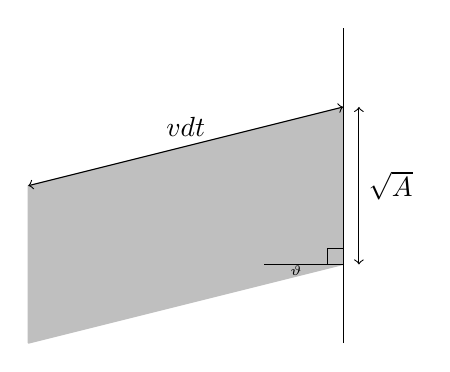
\begin{tikzpicture}
            %\draw[lightgray] (0, 0) grid (5, 5);
            \draw[fill=lightgray, color=lightgray] (0, 0) -- (4, 1) -- (4, 3) -- (0, 2) -- (0, 0);
            \draw (4, 0) -- (4, 4);
            \draw (4, 1) -- (3, 1);
            \node at (3.4, 0.92) {\tiny{\(\vartheta\)}};
            \draw (4, 1) rectangle (3.8, 1.2);
            \draw[<->] (0, 2) -- (4, 3);
            \node[above] at (2, 2.5) {\(vdt\)};
            \draw[<->] (4.2, 1) -- (4.2, 3);
            \node[right] at (4.2, 2) {\(\sqrt{A}\)};
        \end{tikzpicture}
        \caption{Molecules travelling at speed \(v\) at an angle \(\vartheta\) to the surface normal will hit the wall in time \(dt\) if they are in the shaded box.}
        \label{fig:molecules that will hit the wall}
    \end{figure}
    The volume of the box is \(Avdt\cos\vartheta\).
    The number of molecules per unit volume which have speeds \(v\to v+dv\) and angles to the surface normal \(\vartheta\to\vartheta + d\vartheta\) is
    \[n\left(\frac{1}{2}\sin\vartheta d\vartheta\right)f(v)dv\]
    The first term \(n\) accounts for the number of molecules per unit volume, the second term \(\sin\vartheta d\vartheta/2\) accounts for the fraction of molecules with the desired angle and the final term \(f(v)dv\) accounts for the fraction of molecules that have the desired speed.
    The number of impacts in an area \(A\) in time interval \(dt\) is given by
    \[Avdt\cos\vartheta n\left(\frac{1}{2}\sin\vartheta d\vartheta\right)f(v)dv\]
    The flux \(\Phi\) is the number of impacts per unit area per unit time.
    The flux due to molecules travelling at speed \(v\) at angle \(\vartheta\) is \(d\Phi_{v\vartheta}\) and is given by
    \[d\Phi_{v\vartheta} = n(v\cos\vartheta)\frac{1}{2}\sin\vartheta d\vartheta f(v)dv\]
    The pressure is the force per area which by Newton's second law is the change of momentum per area which is
    \[dp = 2mv\cos\vartheta d\Phi_{v,\vartheta}\]
    Where the term \(2mv\cos\vartheta\) accounts for the change in momentum per collision and the flux accounts for the number of collisions per unit area.
    \[dp = nm\sin\vartheta\cos^2\vartheta d\vartheta v^2f(v)dv\]
    \[p = nm\int_0^{\pi/2}\sin\vartheta\cos^2\vartheta\, d\vartheta \int_0^\infty v^2f(v)\,dv\]
    \[I = \int_0^{\pi/2}\sin\vartheta\cos^2\vartheta\, d\vartheta\]
    \[\dv{(\cos\vartheta)}{\vartheta} = -\sin\vartheta \implies d\vartheta = \frac{d(\cos\vartheta)}{-\sin\vartheta}\]
    \[\implies I = \int_{\vartheta = 0}^{\vartheta = \pi/2}\sin\vartheta\cos^2\vartheta\frac{d(\cos\vartheta)}{-\sin\vartheta} = \int_{\vartheta = 0}^{\vartheta = \pi/2}-\cos^2\vartheta\,d(\cos\vartheta)\]
    \[\implies I = \left[-\frac{1}{3}\cos^3\vartheta\right]_{\vartheta = 0}^{\vartheta = \pi/2} = \frac{1}{3}\left(-\cos^3 \frac{\pi}{2} + \cos^3 0\right) = \frac{1}{3}\]
    \[\int_0^\infty v^2f(v)\,dv = \expected{v^2}\]
    \[p = \frac{1}{3}nm\expected{v^2}\]
    We can use the facts that \(n = N/V\) and \(\expected{v^2} = 3k_BT/m\) to write the pressure as
    \[p = nk_BT\]
    \[pV = Nk_BT\]
    \[p = \frac{2\expected{E_K}}{3V}\]
    the last one means that we can think of the pressure of an ideal gas as the kinetic energy density (times a constant 2/3).
    
    \subsection{Effusion}
    We can now come back to the process of effusion.
    The rate of effusion through a small hole area \(A\) is given by
    \[\Phi A\]
    where \(\Phi\) is the total flux.
    \[\Phi = \frac{n}{2}\int_0^{\pi/2}\sin\vartheta\cos\vartheta\, d\vartheta \int_0^{\infty}v f(v)\,dv\]
    \[= \frac{n\expected{v}}{2}\frac{1}{2}\int_0^{\pi/2}\sin 2\vartheta\, d\vartheta\]
    \[= \frac{n\expected{v}}{4}\left[-\frac{\cos 2\vartheta}{2}\right]_0^{\pi/2} = \frac{n\expected v}{4}\]
    \[\Phi = \frac{p}{\sqrt{2\pi mk_BT}}\]
    The fact that \(p\propto 1/\sqrt{m}\) is known as Graham's law.
    It was used in the Manhattan project to separate \ce{^{238}UF_6} and \ce{^{235}UF_6}.
    
    The molecules that start at a distance \(v \cos\vartheta dt\) from the hole will escape in a time \(dt\) if \(\vartheta \in [0, \pi/2]\).
    The number escaping per unit time per area of hole is
    \[d\Phi_{v\vartheta} = n v\cos\vartheta \frac{1}{2}\sin\vartheta d\vartheta f(v)dv\]
    The extra factor of \(v\) at the start is important.
    When considering the kinetic energies of the particles we must consider this factor of \(v\) for example the average kinetic energy of escaping molecules is
    \[\expected{E_K} = \frac{\int_0^\infty v^3f(v)\,dv}{\int_0^\infty vf(v)\,dv} = 2k_BT\]
    Notice that it is \(v^3f(v)\) and \(vf(v)\) in the integrands that would normally just be \(v^2f(v)\) and \(f(v)\).
    The angle integrals are the same in the numerator and denominator so cancel.
    The faster moving molecules (higher temperature) are more likely to escape.
    
    \subsection{Exponential Atmosphere}
    From section \ref{sec:boltzmann factor} we saw that
    \[P \propto e^{-E/k_BT}\]
    We will use this to approximate the air pressure at the peak of Mount Everest.
    We are interested in a change in height so the relevant energy is gravitational potential energy.
    \[mgh\sim \SI{4e-21}{J}\]
    where \(h = \SI{8.8}{km}\) is the height of Mount Everest.
    By coincidence at standard temperatures \(k_BT \sim \SI{4e-21}{J}\) so the number of molecules per unit volume at the peak is
    \[n = n_0\exp\left(-\frac{mgh}{k_BT}\right) = n_0e^{-1}\]
    where \(n_0\) is the number of particles per molecule at sea level
    Since the number of molecules is proportional to the pressure
    \[p = p_0e^{-1} \approx \SI{3.7e4}{Pa}\]
    
    We can make the same prediction with (mostly) macroscopic physics.
    We assume a constant temperature (isothermal atmosphere).
    The hydrostatic pressure change \(dp\) due to a fluid of density \(\rho\) over a height \(dh\) is
    \[dp = -\rho g dh\]
    We consider a gas in a cylinder supporting a piston with its underside at height \(h\) and its top surface at height \(h + dh\).
    We must allow some method for the gas below the piston and above to reach a thermal equilibrium.
    The pressure difference times the area of the piston must be equal to the force due to the displacement of gas upwards by the piston:
    \[(p - (p + dp))A = n(Adh)mg\]
    The first two terms on the left hand side give the pressure below and above the piston.
    \[-\dv{p}{h} = nmg\]
    \[p = nk_BT\]
    \[dp = -\frac{mg}{k_BT}dh\]
    \[p = p_0\exp\left(-\frac{mgh}{k_BT}\right)\]
    So we get the same result if we make the same assumptions required for the Maxwell--Boltzmann distribution, ie isothermal atmosphere and equilibrium.
    
    \section{Transport}
    Some properties of fluids can be thought of as transport of something:
    \begin{itemize}
        \item Diffusion is transport of molecules
        \item Viscosity is transport of momentum
        \item Thermal conductivity is transport of heat
    \end{itemize}
    These processes are all driven by a gradient, for these cases the gradient is concentration, velocity and temperature respectively.
    
    \subsection{Mean Free Path}
    The key length scale in all of these cases is the mean free path length \(\lambda\).
    It is the average distance between molecular collisions.
    To find \(\lambda\) consider a frame where all but one particle is stationary.
    The moving molecule sweeps out an imaginary collision tube.
    If the centre of another molecule is in this tube then it will collide with the moving molecule.
    The cross sectional area \(\sigma\) of this tube is
    \[\sigma = \pi(a_1 + a_2)^2\]
    where \(a_1\) is the radius of the moving molecule and \(a_2\) is the radius of all of the other molecules.
    This follows from the fact that two spheres will overlap if and only if the distance between them is less than or equal to the sum of their radii.
    In time \(t\) the molecule collides with \(\sigma v tn\) molecules where we use \(v = \expected{v_r}\) as the average velocity of the moving molecule relative to the other molecules.
    The molecule also travels a distance of \(\expected{v}t\).
    This gives us the mean free path length as the length of the path divided by the number of collisions:
    \[\lambda = \frac{\expected vt}{\sigma\expected{v_r}tn}\]
    For the Maxwell--Boltzmann distribution we can make an approximation of \(\expected{v_r}\).
    For this distribution we have
    \[\frac{\expected{v}}{\sqrt{\expected{v^2}}} = \sqrt{\frac{8}{3\pi}} = 0.92 \approx 1\]
    so we can approximate \(\expected{v} \approx \sqrt{\expected{v^2}}\) that is we can approximate the mean as the root mean square.
    We can thus approximate \(\expected{v_r} \approx \sqrt{\expected{v_r^2}}\).
    We now consider two molecules with velocities \(\vv v_1\) and \(\vv v_2\).
    This gives us a relative velocity
    \[\vv v_r = \vv v_1 - \vv v_2\]
    \[v_r^2 = \vv v_r\cdot\vv v_r = (\vv v_1 - \vv v_2)\cdot(\vv v_1 - \vv v_2) = v_1^2 + v_2^2 - 2\vv v_1\cdot\vv v_2\]
    \[\expected{v_r^2} = \expected{v_1^2} + \expected{v_2^2} - 2\expected{\vv v_1\cdot\vv v_2}\]
    Since all directions are equally likely \(\expected{\vv v_1\cdot\vv v_2} = 0\), as well as this \(\expected{v_1^2} = \expected{v_2^2} = \expected{v^2}\)
    \[\expected{v_r^2} = 2\expected{v^2}\]
    \[\expected{v_r}\approx\sqrt{\expected{v_r^2}} = \sqrt{2\expected{v^2}}\approx\expected{v}\sqrt{2}\]
    so we can approximate \(\expected{v_r}\approx\expected{v}\sqrt{2}\).
    Going back to the mean free path length we can now write this as
    \[\lambda = \frac{\expected{v}t}{\sigma\expected{v}\sqrt{2}tn} = \frac{1}{\sigma n\sqrt{2}}\]
    We can use \(p = nk_BT\) to write this as
    \[\lambda = \frac{k_BT}{p\sigma\sqrt{2}}\]
    From this it is clear that increasing pressures decreases \(\lambda\).
    This is because the molecules become closer together on average so more collisions occur in the same time.
    
    For this derivation we have assumed that there are no intermolecular forces.
    If there where then they would simply have the effect of increasing the effective collision cross section as the molecules would no longer need to actually touch to collide but just come close to each other.
    
    \example
    What is the mean free path length of \ce{N2} at \SI{300}{K} and \SI{e5}{Pa}?
    The molecular diameter \(d\) is \(d = \SI{0.37}{nm}\).
    This gives a cross section \(\sigma = \pi d^2 = \SI{4.3e-19}{m^2}\).
    The mean free path is then \(\lambda = \SI{6.8e-8}{m}\).
    
    In general the mean free path \(\lambda\approx \SI{100}{nm}\).
    For comparison the average intermolecular separation is \(\expected{s} \approx \SI{4}{nm}\) and the molecular diameter is usually about \(d = \SI{0.4}{nm}\).
    The time \(\tau\) between collisions is
    \[\tau = \frac{\lambda}{\expected v} \approx \SI{0.14}{ns}\]
    
    \subsection{Diffusion}
    Diffusion is transport of molecules driven by a concentration gradient.
    Molecules spread away from an area of high concentration.
    We will start by considering one dimensional random walks.
    If all of the volume of fluid is split by planes area \(A\) into bins then we define \(N(z)\) to be the number of molecules in the bin containing the point \(z\).
    If all of the planes are a distance \(L\) apart then the number of molecules in the plane to the left of the plane containing \(z\) is \(N(z - L)\).
    \begin{figure}[ht]
        \centering
        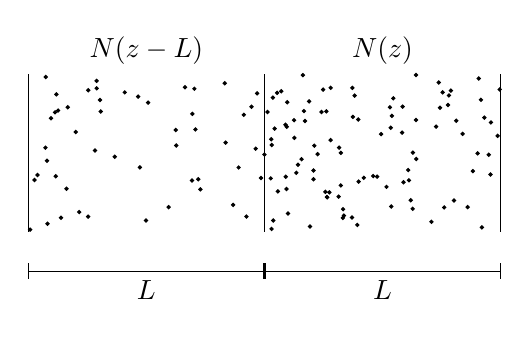
\begin{tikzpicture}
            \draw (0, 0) -- (0, 2);
            \draw (3, 0) -- (3, 2);
            \draw (6, 0) -- (6, 2);
            \draw[|-|] (0, -0.5) -- (3, -0.5);
            \draw[|-|] (3, -0.5) -- (6, -0.5);
            \node[below] at (1.5, -0.5) {\(L\)};
            \node[below] at (4.5, -0.5) {\(L\)};
            \node[above] at (1.5, 2) {\(N(z - L)\)};
            \node[above] at (4.5, 2) {\(N(z)\)};
            
            \draw[fill=black] (2.738, 1.486) circle (0.02cm);\draw[fill=black] (0.025, 0.028) circle (0.02cm);\draw[fill=black] (0.921, 1.527) circle (0.02cm);\draw[fill=black] (1.783, 0.313) circle (0.02cm);\draw[fill=black] (0.239, 0.902) circle (0.02cm);\draw[fill=black] (0.647, 0.251) circle (0.02cm);\draw[fill=black] (0.868, 1.917) circle (0.02cm);\draw[fill=black] (1.992, 1.836) circle (0.02cm);\draw[fill=black] (0.912, 1.675) circle (0.02cm);\draw[fill=black] (0.761, 1.798) circle (0.02cm);\draw[fill=black] (0.223, 1.966) circle (0.02cm);\draw[fill=black] (0.29, 1.442) circle (0.02cm);\draw[fill=black] (1.098, 0.954) circle (0.02cm);\draw[fill=black] (2.602, 0.342) circle (0.02cm);\draw[fill=black] (0.486, 0.548) circle (0.02cm);\draw[fill=black] (0.502, 1.581) circle (0.02cm);\draw[fill=black] (0.379, 1.54) circle (0.02cm);\draw[fill=black] (0.35, 0.706) circle (0.02cm);\draw[fill=black] (2.889, 1.056) circle (0.02cm);\draw[fill=black] (2.907, 1.759) circle (0.02cm);\draw[fill=black] (0.118, 0.721) circle (0.02cm);\draw[fill=black] (1.418, 0.818) circle (0.02cm);\draw[fill=black] (0.341, 1.518) circle (0.02cm);\draw[fill=black] (0.358, 1.746) circle (0.02cm);\draw[fill=black] (1.396, 1.718) circle (0.02cm);\draw[fill=black] (0.417, 0.179) circle (0.02cm);\draw[fill=black] (0.079, 0.658) circle (0.02cm);\draw[fill=black] (1.522, 1.641) circle (0.02cm);\draw[fill=black] (2.956, 0.683) circle (0.02cm);\draw[fill=black] (2.672, 0.817) circle (0.02cm);\draw[fill=black] (2.497, 1.887) circle (0.02cm);\draw[fill=black] (0.218, 1.068) circle (0.02cm);\draw[fill=black] (1.873, 1.293) circle (0.02cm);\draw[fill=black] (0.604, 1.268) circle (0.02cm);\draw[fill=black] (0.245, 0.103) circle (0.02cm);\draw[fill=black] (1.88, 1.096) circle (0.02cm);\draw[fill=black] (2.123, 1.3) circle (0.02cm);\draw[fill=black] (2.084, 1.498) circle (0.02cm);\draw[fill=black] (2.506, 1.133) circle (0.02cm);\draw[fill=black] (2.836, 1.589) circle (0.02cm);\draw[fill=black] (1.226, 1.771) circle (0.02cm);\draw[fill=black] (1.495, 0.144) circle (0.02cm);\draw[fill=black] (2.187, 0.539) circle (0.02cm);\draw[fill=black] (0.87, 1.822) circle (0.02cm);\draw[fill=black] (0.761, 0.193) circle (0.02cm);\draw[fill=black] (2.159, 0.668) circle (0.02cm);\draw[fill=black] (2.079, 0.652) circle (0.02cm);\draw[fill=black] (0.847, 1.033) circle (0.02cm);\draw[fill=black] (2.771, 0.194) circle (0.02cm);\draw[fill=black] (2.11, 1.817) circle (0.02cm);\draw[fill=black] (3.283, 1.335) circle (0.02cm);\draw[fill=black] (5.263, 1.772) circle (0.02cm);\draw[fill=black] (3.27, 0.699) circle (0.02cm);\draw[fill=black] (3.489, 1.99) circle (0.02cm);\draw[fill=black] (3.745, 1.807) circle (0.02cm);\draw[fill=black] (3.97, 1.003) circle (0.02cm);\draw[fill=black] (3.28, 0.545) circle (0.02cm);\draw[fill=black] (5.435, 1.411) circle (0.02cm);\draw[fill=black] (5.179, 1.336) circle (0.02cm);\draw[fill=black] (5.408, 0.398) circle (0.02cm);\draw[fill=black] (3.793, 0.442) circle (0.02cm);\draw[fill=black] (5.343, 1.732) circle (0.02cm);\draw[fill=black] (3.578, 0.067) circle (0.02cm);\draw[fill=black] (3.567, 1.656) circle (0.02cm);\draw[fill=black] (3.97, 0.589) circle (0.02cm);\draw[fill=black] (4.123, 1.46) circle (0.02cm);\draw[fill=black] (3.84, 1.165) circle (0.02cm);\draw[fill=black] (3.376, 1.418) circle (0.02cm);\draw[fill=black] (3.267, 1.359) circle (0.02cm);\draw[fill=black] (3.774, 0.508) circle (0.02cm);\draw[fill=black] (5.707, 0.997) circle (0.02cm);\draw[fill=black] (5.229, 1.575) circle (0.02cm);\draw[fill=black] (3.675, 0.986) circle (0.02cm);\draw[fill=black] (5.516, 1.244) circle (0.02cm);\draw[fill=black] (3.161, 1.766) circle (0.02cm);\draw[fill=black] (4.858, 0.401) circle (0.02cm);\draw[fill=black] (3.515, 1.408) circle (0.02cm);\draw[fill=black] (4.882, 0.293) circle (0.02cm);\draw[fill=black] (3.942, 0.447) circle (0.02cm);\draw[fill=black] (3.039, 1.521) circle (0.02cm);\draw[fill=black] (4.825, 0.785) circle (0.02cm);\draw[fill=black] (5.876, 1.389) circle (0.02cm);\draw[fill=black] (5.871, 0.728) circle (0.02cm);\draw[fill=black] (3.0, 0.981) circle (0.02cm);\draw[fill=black] (4.619, 1.473) circle (0.02cm);\draw[fill=black] (5.33, 1.611) circle (0.02cm);\draw[fill=black] (5.213, 1.897) circle (0.02cm);\draw[fill=black] (3.996, 0.176) circle (0.02cm);\draw[fill=black] (3.502, 1.533) circle (0.02cm);\draw[fill=black] (3.38, 1.194) circle (0.02cm);\draw[fill=black] (4.192, 1.426) circle (0.02cm);\draw[fill=black] (5.749, 1.677) circle (0.02cm);\draw[fill=black] (4.481, 1.241) circle (0.02cm);\draw[fill=black] (4.748, 1.26) circle (0.02cm);\draw[fill=black] (4.928, 0.926) circle (0.02cm);\draw[fill=black] (3.797, 0.438) circle (0.02cm);\draw[fill=black] (4.637, 1.696) circle (0.02cm);\draw[fill=black] (4.61, 0.322) circle (0.02cm);\draw[fill=black] (4.009, 0.207) circle (0.02cm);\draw[fill=black] (5.121, 0.127) circle (0.02cm);\draw[fill=black] (3.289, 1.646) circle (0.02cm);\draw[fill=black] (5.647, 0.771) circle (0.02cm);\draw[fill=black] (5.581, 0.314) circle (0.02cm);\draw[fill=black] (4.886, 1.006) circle (0.02cm);\draw[fill=black] (4.116, 1.828) circle (0.02cm);\draw[fill=black] (4.835, 0.654) circle (0.02cm);\draw[fill=black] (3.106, 1.704) circle (0.02cm);\draw[fill=black] (3.08, 0.679) circle (0.02cm);\draw[fill=black] (3.09, 0.037) circle (0.02cm);\draw[fill=black] (3.623, 0.779) circle (0.02cm);\draw[fill=black] (3.405, 0.75) circle (0.02cm);\draw[fill=black] (3.093, 1.103) circle (0.02cm);\draw[fill=black] (5.849, 0.978) circle (0.02cm);\draw[fill=black] (4.112, 0.183) circle (0.02cm);\draw[fill=black] (3.999, 0.287) circle (0.02cm);\draw[fill=black] (4.381, 0.708) circle (0.02cm);\draw[fill=black] (4.179, 0.088) circle (0.02cm);\draw[fill=black] (4.593, 1.582) circle (0.02cm);\draw[fill=black] (3.17, 0.513) circle (0.02cm);\draw[fill=black] (3.633, 1.094) circle (0.02cm);\draw[fill=black] (4.754, 1.59) circle (0.02cm);\draw[fill=black] (3.786, 1.53) circle (0.02cm);\draw[fill=black] (3.426, 0.851) circle (0.02cm);\draw[fill=black] (4.925, 1.991) circle (0.02cm);\draw[fill=black] (4.766, 0.63) circle (0.02cm);\draw[fill=black] (3.471, 0.923) circle (0.02cm);\draw[fill=black] (5.987, 1.808) circle (0.02cm);\draw[fill=black] (3.112, 0.144) circle (0.02cm);\draw[fill=black] (3.299, 0.234) circle (0.02cm);\draw[fill=black] (3.213, 1.786) circle (0.02cm);\draw[fill=black] (5.722, 1.948) circle (0.02cm);\draw[fill=black] (4.196, 0.638) circle (0.02cm);\draw[fill=black] (5.762, 0.056) circle (0.02cm);\draw[fill=black] (3.623, 0.668) circle (0.02cm);\draw[fill=black] (3.824, 0.501) circle (0.02cm);\draw[fill=black] (3.086, 1.175) circle (0.02cm);\draw[fill=black] (4.604, 1.321) circle (0.02cm);\draw[fill=black] (3.724, 1.522) circle (0.02cm);\draw[fill=black] (3.129, 1.311) circle (0.02cm);\draw[fill=black] (3.841, 1.829) circle (0.02cm);\draw[fill=black] (4.925, 1.421) circle (0.02cm);\draw[fill=black] (5.962, 1.219) circle (0.02cm);\draw[fill=black] (4.146, 1.73) circle (0.02cm);\draw[fill=black] (3.948, 1.069) circle (0.02cm);\draw[fill=black] (4.55, 0.571) circle (0.02cm);\draw[fill=black] (5.792, 1.45) circle (0.02cm);\draw[fill=black] (4.262, 0.686) circle (0.02cm);\draw[fill=black] (5.283, 0.31) circle (0.02cm);\draw[fill=black] (5.368, 1.794) circle (0.02cm);\draw[fill=black] (4.432, 0.701) circle (0.02cm);
        \end{tikzpicture}
        \caption{Gas divided into bins width \(L\) containing \(N\) molecules}
    \end{figure}
    The volume of a bin is \(LA\) if the number density of the fluid defusing is \(n^*\) then \(N = ALn^*\).
    If in time \(\tau\) half the molecules step from left to right an half step from right to left then the net nuber crossing from left to right is given by
    \[\frac{1}{2}(N(z - L) - N(z)) = \frac{L}{2}\dv{N}{z}\]
    The flux \(\Phi\) is given by
    \begin{equation}\label{eqn:flux = -diffusion * dn/dz}
        \Phi = -\frac{L}{2A\tau}\dv{N}{z} = -\frac{L^2}{2\tau}\dv{n^*}{z} = -D\dv{n^*}{z}
    \end{equation}
    We can identify that \(L\leftrightarrow\lambda\) since this is the length of one step.
    \(D\) is the diffusion coefficient.
    
    \subsection{Diffusion Coefficient and Fick's Law}
    \begin{figure}[ht]
        \centering
        \begin{tikzpicture}
            \draw (0, 0) -- (4, 0) -- (4, 4) -- (0, 4) -- (0, 0);
            \draw[color=lightgray] (2, 0) -- (2, 1.9);
            \draw[color=lightgray] (2, 4) -- (2, 2.1);
            \draw[dashed] (2, 2) circle (1cm);
            \draw (2, 2) -- (1, 2);
            \draw (2, 2) -- (1.292, 1.292);
            \node[below left] at (1.9, 2.05) {\tiny \(\vartheta\)};
            \node[above] at (1.5, 2) {\tiny\(\lambda\)};
            \node[below] at (2, 0) {\(W\)};
            \node[below] at (1, 0) {\(L\)};
            \node[below] at (3, 0) {\(R\)};
            \draw[->] (0, 4.2) -- (4, 4.2);
            \node[right] at (4, 4.2) {\(z\)};
        \end{tikzpicture}
        \caption{Concentration gradient decreases from left to right.}
        \label{fig:window}
    \end{figure}
    Figure \ref{fig:window} shows a box with a concentration gradient.
    We place an imaginary window in the plane dividing the box in half at \(W\).
    Recall that \(\Phi\propto n^*\).
    One question that we can ask is how much higher is the concentration at \(L\) than at \(R\)?
    This depends on the positions of \(L\) and \(R\) and also on the value of \(\partial_z n^*\).
    The last change in direction of a particle before it went through the window must have occurred somewhere on the circle if we assume all steps are of size \(\lambda\).
    This means that it occurred at a distance \(\lambda\cos\vartheta\) along the \(z\) axis.
    The excess concentration at \(L\) is
    \[-\lambda\cos\vartheta\partial_z n^*\]
    The flux approaching \(W\) from the left exceeds that leaving by the right by
    \[d\Phi_{\vartheta v} = -\pdv{n^*}{z}\lambda\cos\vartheta\frac{1}{2}sin\vartheta\cos\vartheta d\vartheta vf(v)dv\]
    The total excess flux is
    \[\Phi_z = -\frac{1}{2}\pdv{n^*}{z}\lambda\int_0^\pi \cos^2\vartheta\sin\vartheta\,d\vartheta\int_0^\infty vf(v)\,dv\]
    \[\Phi_z = -\frac{\lambda}{3}\expected{v}\pdv{n^*}{z}\]
    This last line is Fick's law.
    From this we can equate with equation \ref{eqn:flux = -diffusion * dn/dz} and we get
    \[D = \frac{\lambda}{3}\expected{v}\]
    \[[D] = \si{m^2.s^{-1}},\qquad D\propto p^{-1} \propto T^{3/2},\qquad \expected{v} \propto T^{1/2}\]
    Diffusion is faster at higher temperatures as the particles are faster and at lower pressures as the mean free path is longer.
    
    We can treat diffusion as a large number of random walks.
    The expected square of the length of an \(N\) step walk of step length \(l\) is \(\expected{x_N^2} = Nl^2\).
    The step size \(l = \lambda\) and in time \(t\) the number of steps is given by the number of collisions so \(N = t\expected{v}/\lambda\).
    \[\expected{x_N^2} = \expected{v}\lambda t\]
    \[D = \frac{\lambda}{3}\expected{v}\]
    \[\sqrt{{x_N^2}} \propto \sqrt{Dt}\]
    we can take \(\sqrt{x_N^2}\) as a measure of the width of the distribution so we can also do the same with \(\sqrt{Dt}\).
    So if \(D\) is very high or after a long time we would expect the distribution to look wide and flat as the gas is evenly spread.
    If \(D\) is very low or for small \(t\) we would expect a sharp distribution with all the gas in one place.
    
    We used the molecular diameter to construct this entire argument but we can work back and measure \(D\) to get \(d\).
    When we do this we find that the value of \(d\) is in agreement with other methods such as those that depend on different transport properties.
    This was important evidence for the molecular nature of matter early on in statistical mechanics.
    
    \subsection{Viscosity}
    Consider two plates area \(A\) sandwiching a fluid.
    The top plate moves with velocity \(u\) relative to the bottom plate.
    This establishes a velocity gradient as the fluid near a wall has a velocity that matches that of the wall.
    We imagine the fluid as a series of layers.
    Molecules in the layer next to the top plate will collide with the layer below and in doing so lose some momentum and cause the layer below to gain some.
    Like wise molecules in the lowest layer will collide with molecules in the layer above and gain some of their momentum.
    In this way momentum is transferred from the top plate to the bottom plate.
    
    \begin{figure}[ht]
        \centering
        \begin{tikzpicture}
            \draw (0, 0) -- (6, 0);
            \draw (0, 4) -- (6, 4);
            \draw[dashed] (2, 0) -- (2, 4);
            \draw[dashed] (2, 0) -- (4, 4);
            \draw[->] (2, 1) -- (2.5, 1);
            \draw[->] (2, 2) -- (3, 2);
            \draw[->] (2, 3) -- (3.5, 3);
            \node[right] at (3, 2) {\(\expected{u_x}\)};
            \draw[<->] (5, 3) -- (5, 2) -- (6, 2);
            \node[above] at (5, 3) {\(z\)};
            \node[right] at (6, 2) {\(x\)};
        \end{tikzpicture}
        \caption{Velocity Gradient}
    \end{figure}
    
    We define the shear stress \(\tau_{xz}\) to be the force per unit area which is equivalently the flux of momentum which is in turn the rate of transfer of momentum per unit area.
    The flux is given by
    \[d\Phi_{v\vartheta} = \frac{1}{2}\sin\vartheta\cos\vartheta d\vartheta nvf(v)dv\]
    A molecule a distance \(\lambda\cos\vartheta\) up the velocity gradient carries additional momentum given by
    \[-m\pdv{\expected{u_x}}{z}\lambda\cos\vartheta\]
    where \(\expected{u_x}\) is the average velocity in the \(x\) at a heigh \(z\) and \(m\) is the mass of the .
    The flux of the momentum is then given by
    \[\Phi = -\frac{1}{2}nm\lambda\pdv{\expected{u_x}}{z}\int_0^\pi\cos^2\vartheta\sin\vartheta\, d\vartheta\int_0^\infty vf(v)\,dv\]
    \[\Phi = -\frac{1}{3}nm\lambda\expected{v}\pdv{\expected{u_x}}{z}\]
    We define the viscosity \(\eta\) to be
    \[\eta = \frac{1}{3}nm\lambda\expected{v}\]
    which allows us to write
    \[\tau_{xz} = \eta\dv{\expected{u_x}}{z}\]
    We can substitute in
    \[\lambda = \frac{1}{\sigma n\sqrt 2}\]
    to get
    \[\eta = \frac{1}{3}\frac{nm}{\sigma n\sqrt 2} = \frac{\sqrt 2}{6}\frac{m}{\sigma}\expected{v}\]
    we see that \(\eta\) is independent of \(n\) and hence independent of pressure.
    This is because when the pressure increases the number of collisions increases but the efficacy of the collisions transferring momentum decreases and these effects cancel out.
    For a gas \(\eta\propto\sqrt T\) so increasing temperature increases the viscosity.
    For most liquids increasing temperature decreases velocity.
    
    \section{Thermodynamics}
    \subsection{Heat Flux}
    The flux of heat is given by
    \[\frac{1}{A}\dv{Q}{T} = -\kappa\dv{T}{y}\]
    where
    \[\kappa = \frac{1}{3}n\expected{v}\lambda C_\text{molecule}\]
    Where \(Q\) is the heat, \(A\) is the area and \(C_\text{molecule}\) is the heat capacity of one molecule.
    Since the temperature is related to the average kinetic energy then a transfer of kinetic energy by collision is related to a transfer of heat and hence the mechanism for temperature transfer is collisions.
    
    \subsection{What is Thermodynamics}
    Thermodynamics connects energy, heat work and temperature.
    Classical thermodynamics as a framework was established before the molecular nature of matter was widely accepted.
    Statistical thermodynamics was established after.
    We will be using which ever is more convenient in this course.
    Thermodynamics is interested in how macroscopic variables are related.
    
    \subsection{Zeroth Law of Thermodynamics}
    The zeroth law was added after the other three laws when it became clear that a definition of thermal equilibrium was needed.
    Two bodies are defined to be in thermal equilibrium if they are the same temperature.
    The zeroth law states
    \begin{displayquote}
        Two bodies \(A\) and \(B\) that are separately in thermal equilibrium with a third body \(C\) they are also in thermal equilibrium with each other.
    \end{displayquote}
    Thermal equilibrium is an equivalence relation since all objects are in thermal equilibrium with themselves, thermal equilibrium is symmetric and the zeroth law states the transitivity of thermal equilibrium.
    
    This law is the basis for how thermometers work since they are calibrated from one object and then allowed to reach a thermal equilibrium with another. 
    Then they give the temperature under the assumption that the calibration object and object being measured are in thermal equilibrium if the associated pressure change in the thermometer is the same.
    
    If two systems are in thermal contact then there will be an energy transfer, on average, from the hotter object of temperature \(T_2\) to the cooler object of temperature \(T_1\) and eventually thermal equilibrium will be achieved.
    The temperature \(T\) at thermal equilibrium will be \(T_1 < T < T_2\).
    
    \subsection{First Law of Thermodynamics}
    Joule did experiments where he did work on a system in various ways, for example dropping a weight or with an electric current.
    He observed that the heat transfer is the same for the same amount of work.
    This established that heat and work are equivalent ways of increasing the internal energy of a system.
    
    Heat \(Q\) is thermal energy in transit.
    Work \(W\) is also energy in transit but it is motion against a force.
    Work is done  if the process could be used to change the height of a weight.
    If the weight is raised work is done by the system.
    If the weight is lowered work is done on the system.
    An important distinction is that heat is transfer of energy by disorderly thermal motion whereas work is transfer of energy by organised motion.
    
    Energy is the capacity to do work.
    Internal energy \(U\) is the total energy of all internal degrees of freedom that the system possesses.
    The internal energy is the sum of the kinetic and potential energies.
    
    A state function depends only on the condition of the system.
    A path function depends on how the system got into that state.
    
    Internal energy change \(\Delta U = U_f - U_i\) is a state function.
    The first law of thermodynamics is
    \begin{displayquote}
        If a system absorbs heat \(Q\) and work \(W\) is done on the system then the change in internal energy is
        \[\Delta U = Q + W\]
    \end{displayquote}
    This is often written in terms of infinitesimal changes:
    \[dU = dQ + dW\]
    
    \subsubsection{Work done in Gas Expansion}
    A piston area \(A\) is compressed by a force \(F\) due to an external pressure \(p_\text{ext}\).
    The piston moves a distance \(dx\).
    What is the work done?
    
    We consider the external pressure to be a constant.
    The force is given by
    \[F = p_\text{ext}A\]
    The work done is then
    \[dW = Fdx\]
    \[dW = p_\text{ext}Adx\]
    The change in volume of the gas in the piston is
    \[dV = -Adx\]
    where the negative denotes a decrease in volume.
    Hence the work done is
    \[dW = -p_\text{ext}dV\]
    \[W = -p_\text{ext}\int_{V_i}^{V_f}dV = -p_\text{ext}[V_f - V_i]\]
    If the gas is compressed then the work is positive and we say work has been done on the gas in the piston.
    The internal energy of the gas in the piston increases and its temperature increases.
    
    If we consider work done in a reversible isothermal (constant temperature) expansion. A reversible change is one that can be reversed by an infinitesimal change in a variable.
    If the internal pressure is only infinitesimally greater than the external pressure then the piston moves out infinitely slowly and the motion can be reversed by an infinitesimal increase in the external pressure.
    The pressures are balanced so the system is always at equilibrium.
    In this case we can ensure reversibility by setting \(p_\text{int} = p_\text{ext}\).
    
    The pressure of the gas in the piston is
    \[p_\text{int} = \frac{n_mRT}{V}\]
    for an ideal gas.
    The work done is
    \[dW = -p_\text{ext}\dd V\]
    \[W = -\int_{V_i}^{V_f}p_\text{int}\,dV = -n_mRT\int_{V_i}^{V_f}\frac{1}{V}\,dV = -n_mRT\ln\left(\frac{V_f}{V_i}\right)\]
    
    Work done reversibly is a maximum.
    At higher temperatures if everything else is unchanged more work will be done.
    For an ideal gas undergoing an isothermal change since all energy is kinetic \(\Delta U = 0\).
    The heat transfer in this case is
    \[Q = -W = n_mRT\ln\left(\frac{V_f}{V_i}\right)\]
    In an adiabatic process no heat is transferred so \(Q = 0\).
    The temperature can still change if the volume or pressure changes.
    We can approximate the work done as somewhere between the work done in an isothermal change at the start temperature and the work done in an isothermal change at the final temperature.
    
    \subsection{Heat Capacity}
    We define the heat capacity, \(C\), of an object as
    \[C = \dv{Q}{T}\]
    We generally consider two different cases where we want to know the heat capacity.
    At constant pressure or at constant volume.
    These are denoted with a subscript \(p\) or \(V\) respectively and are defined as
    \[C_p = \pdvconst{Q}{T}{p},\qquad C_V = \pdvconst{Q}{T}{V}\]
    To keep the pressure constant the gas must expand so it has to do work against the atmosphere.
    For this reason we expect that \(C_p > C_V\).
    
    We consider a system where the internal energy is defined by two, independent, thermodynamic variables \(T\) and \(V\) such that \(U = U(T, V)\).
    A small change \((dT, dV)\) in \((T, V)\) will result in a small change \(dU\) in the internal energy:
    \[dU = \pdvconst{U}{T}{V}dT + \pdvconst{U}{V}{T}dV\]
    From before we have the first law \(dU = dQ + dW = dQ - pdV\)
    which allows us to write \(dQ\) as \(dQ = dU + pdV\)
    \begin{align*}
        dQ &= \pdvconst{U}{T}{V}dT + \pdvconst{U}{V}{T}dV + pdV\\
        dQ &= \pdvconst{U}{T}{V}dT + \left[\pdvconst{U}{V}{T} + p\right]dV\\
        \dv{Q}{T} &= \pdvconst{U}{T}{V} + \left[\pdvconst{U}{V}{T} + p\right]\dv{V}{T}\stepcounter{equation}\tag{\theequation}\label{eqn: heat capacity}
    \end{align*}
    At a constant volume the second term is 0 so the first term is equal to \(\mathrm{d}Q/\mathrm{d}T\) and can be identified as the heat capacity at a constant volume.
    \[\dv{Q}{T} = C_V + \left[\pdvconst{U}{V}{T} + p\right]\dv{V}{T}\]
    For an ideal gas all internal energy is kinetic so \(\partial_VU = 0\):
    \[\dv{Q}{T} = C_V + p\dv{V}{T}\]
    For one mole of an ideal gas the volume is
    \[V = \frac{RT}{p}\]
    \[\dv{V}{T} = \frac{R}{p}\]
    \[\dv{Q}{T} = C_V + p\frac{R}{p}\]
    \[\dv{Q}{T} = C_V + R\]
    for one mole of an ideal gas.
    If instead we take equation \ref{eqn: heat capacity} at a constant pressure then we get \(C_p\) instead
    \[C_p = \pdvconst{U}{T}{V} + \left[\pdvconst{U}{V}{T} + p\right]\pdvconst{V}{T}{p}\]
    
    \section{Degrees of Freedom and Entropy}
    \subsection{Quadratic Modes}
    Equipartition applies to any quadratic mode for example the potential energy of a mass on a spring: \(E_p = kx^2/2\).
    For equipartition to apply however the energy of the system must be such that all energy levels are reachable.
    Up to now we have considered ideal, monatomic gases.
    If instead we consider an ideal, diatomic gas then there are more degrees of freedom:
    \begin{itemize}
        \item Translational - There are 3 translational degrees of freedom due to the three different directions a molecule's centre of mass can be translated.
        The quadratic mode here is the kinetic energy associated with this motion.
        The energy levels for translational degrees of freedom are available at any non-zero temperature
        \item Rotational - There are 2 rotational degrees of freedom.
        There are three axis along which rotation is possible but the one that is collinear with the bond results in a very low moment of inertia since only electrons are being rotated so this degree of freedom is actually associated with electron energy levels so isn't considered a rotational degree of freedom.
        The quadratic mode here is the kinetic energy associated with this motion.
        The energy levels for these degrees of freedom are available a temperature of
        \[T = \frac{\hbar^2}{2Ik_B}\]
        where \(I\) is the moment of inertia.
        For a heavy molecule like \ce{Br2} the temperature is \(\sim\SI{20}{K}\).
        For a lighter molecule like \ce{H2} the temperature is \(\sim\SI{100}{K}\).
        \item Vibrational - There are 2 vibrational degrees of freedom.
        The quadratic modes here are the kinetic energy due to the shortening and lengthening of the bond and the potential energy due to this vibration.
        Note that one vibrational mode gives rise to two degrees of freedom.
        The energy levels for these degrees of freedom are available at a temperature of
        \[T = \frac{\hbar\omega}{k_B}\]
        where \(\omega\) is the angular frequency of the vibration.
    \end{itemize}
    The total number of quadratic modes is \(f = 7\).
    At sufficiently high temperatures using equipartition we get
    \[\expected{U} = \frac{7}{2}k_BT\]
    At these same high temperatures for a mole of ideal, diatomic gas
    \[C_V = \frac{7}{2}R = \SI{29.1}{J.K^{-1}.mol^{-1}}\]
    In general for an ideal gas:
    \[C_V = \frac{3}{2}R + \frac{f_\text{rot}}{2}R +  f_\text{vib}R\]
    where \(f_\text{rot}\) and \(f_\text{vib}\) are the number of rotational and vibrational degrees of freedom respectively.
    
    An \(N\) atom molecule has \(3N\) degrees of freedom.
    Of these 3 are translational degrees of freedom.
    If it is linear then there are 2 rotational degrees of freedom and if it is non-linear then there are 3 rotational degrees of freedom.
    The rest are vibrational.
    This gives the number of vibrational degrees of freedom as
    \[f_\text{vib} = 3N - 3 - 2 = 3N - 5\]
    \[f_\text{vib} = 3N - 3 - 3 = 3N - 6\]
    for a linear and non-linear molecule respectively.
    
    \example
    \ce{CO2} has three atoms so it has 9 degrees of freedom.
    It is a linear molecule so it has 3 translational and 2 rotational degrees of freedom.
    It has \(9 - 3 - 2 = 4\) vibrational degrees of freedom.
    One of these is the carbon atom staying stationary while the bonds change length together, one is one bond shortening and the other lengthening and the other two are degenerate and correspond to scissoring of the molecule in two different planes.
    
    \example
    A ratio of \(\gamma = C_p / C_V\) is measured as \(7/5\).
    What can be deduced about the gas?
    \[\gamma = \frac{C_p}{C_V}\ = \frac{C_V + R}{C_V} = 1 + \frac{R}{C_V} = \frac{7}{5}\]
    \[\implies \frac{C_V}{R} = \frac{5}{2}\]
    hence \(C_V = 5R/2\).
    This means that there are 5 degrees of freedom.
    3 degrees of freedom must be translational so there are two rotational degrees of freedom meaning the molecule is linear.
    The fact that there aren't more means that the temperature isn't high enough for the quadratic modes of vibration to be available.
    
    \subsection{Entropy}
    Entropy \(S\) is a measure of the distribution of energy.
    Spontaneous processes increase the number of ways in which energy can be distributed and so increase entropy.
    It is easy to convert work to heat but not the other way around.
    This idea is formalised in the second law of thermodynamics.
    
    \subsection{Second Law of Thermodynamics}
    There have been multiple statements of this law each one improving on the last.
    Clausius stated this law as
    \begin{displayquote}
        No process is possible whose sole result is the transfer of heat from a colder to a hotter body
    \end{displayquote}
    Lord Kelvin improved on this stating
    \begin{displayquote}
        No process is possible whose sole result is the complete conversion of heat into work
    \end{displayquote}
    Now this law is best understood as all processes increase or leave unchanged the entropy of the universe:
    \[\Delta S_\text{univ} \ge 0\]
    We can further split this into two cases.
    If \(\Delta S_\text{univ} > 0\) then the process is spontaneous.
    If \(\Delta S_\text{univ} = 0\) then the process is reversible since the reversal necessarily has equal and opposite entropy change so this must be zero to avoid violating the second law of thermodynamics.
    
    \subsection{Statistical Definition of Entropy}
    Lord Kelvin defined entropy as
    \[S = k_B\ln\Omega\]
    where \(\Omega\) is the number of ways of distributing a fixed number of particles with a fixed amount of energy.
    
    \subsubsection{Joule Expansion of a Gas}
    An ideal gas, at constant temperature, is kept in a container split in to two parts of volume \(V\).
    At first the gas is in one part at pressure \(p_i\) and the other part is a vacuum.
    The boundary is removed.
    What is the change in entropy.
    Say the gas is now at pressure \(p_f\).
    
    Removing the block doubles the number of ways that each molecule could be positioned giving
    \[\frac{\Omega_\text{after}}{\Omega_\text{before}} = 2^{N_A}\]
    \[\Delta S = k_B\ln \Omega_\text{after} - k_B\ln \Omega_\text{before} = k_B\ln\left(\frac{\Omega_\text{after}}{\Omega_\text{before}}\right) = k_B\ln 2^{N_A} = N_Ak_B\ln 2 = R\ln 2\]
    
    \subsection{Thermodynamic Definition of Entropy}
    In thermodynamics entropy is defined in terms of heat transferred in the process if it where reversible even if it isn't.
    For an infinitesimal, reversible, heat transfer \(dQ_\text{rev}\) at temperature \(T\) the entropy change is
    \[dS = \frac{dQ_\text{rev}}{T}\]
    From this definition we can see that entropy is a state function
    
    \subsubsection{Joule Expansion of a Gas}
    We consider the same set up as before but now we use this other definition of entropy to see if we get the same result.
    The expansion is isothermal so \(dU = 0\).
    The first law of thermodynamics \(dU = dQ + dW\) gives us 
    \[0 = dQ + dW\implies dQ = -dW = -(-pdV) = \frac{RT}{V}dV\]
    for one mole of an ideal gas.
    Hence the entropy change is
    \[dS = \frac{dQ_\text{rev}}{T} = \frac{R}{V}dV\]
    \begin{align*}
        \Delta S &= \int_{V_i}^{V_f}\frac{1}{T}\,dQ_\text{rev}\\
        &= R\int_{V_i}^{V_f}\frac{1}{V}\,dV\\
        &= R\ln\left(\frac{V_f}{V_i}\right)\\
        &= R\ln 2
    \end{align*}
    Which is the same result as the statistical method gave us.
    
    \subsection{Surroundings}
    So far we have only considered the entropy change \(\Delta S_\text{sys}\) of the system in question.
    We also need to consider the entropy change \(\Delta S_\text{surr}\) of the surroundings.
    These quantities combined give us the entropy change of the universe
    \[\Delta S_\text{univ} = \Delta S_\text{sys} + \Delta S_\text{surr}\]
    The heat flow from the surroundings \(Q_\text{surr}\) must be equal and opposite to the heat flow \(Q_\text{sys}\) from the system:
    \[Q_\text{surr} = - Q_\text{sys}\]
    The surroundings are the rest of the universe so very big.
    For this reason we can consider heat transfer to the surroundings to be reversible.
    
    Consider a gas expanding reversibly.
    The entropy change of the system is \(\Delta S_\text{sys}\).
    The heat flows from the surroundings to the system.
    The entropy of the surroundings therefore decreases by
    \[\Delta S_\text{surr} = -\int\frac{1}{T}\,dQ_\text{rev} = -\Delta S_\text{sys}\]
    The total entropy change is then
    \[\Delta S_\text{univ} = \Delta S_\text{sys} + \Delta S_\text{surr} = 0\].
    This is a general result for a reversible process.
    
    If instead we consider the Joule expansion as before then since it is isothermal \(\Delta U = 0\).
    No heat is transferred to or from the surroundings so \(Q_\text{rev}^\text{surr} = 0\).
    The entropy change of the surroundings is then 0.
    The entropy change of the system is still \(R\ln 2\).
    \[\Delta S_\text{univ} = \Delta S_\text{sys} + 0 = R\ln 2 > 0\]
    This makes sense as expansion into a vacuum is spontaneous.
    
    %%%%%%%%%%%%%%%%%%%%%%%%%%%%%%%%%%%%%%%%%%%%%%%%%%%%%%%%%%%% ABOVE HERE d needs replacing with \dd
    \section{Enthalpy and Gibbs Free Energy}
    Recall the definition of heat capacity:
    \[C = \dv{Q}{T}\]
    At constant pressure this becomes
    \[C_p = \pdvconst{Q}{T}{p}\implies (\dd Q)_p = C_p\dd T\]
    This gives us an alternative way to write entropy at constant pressure:
    \[\dd S = \frac{\dd Q}{T} = \frac{C_p\dd T}{T}\]
    \[S(T_2) - S(T_2) = \int_{T_1}^{T_2}\dd S = \int_{T_1}^{T_2}\frac{C_p(T)}{T}\,\dd T\]
    At very low temperatures \(C_p \propto T^3\).
    This is Debye's law, we will come back to it later.
    
    \subsection{Third Law of Thermodynamics}
    The third law of thermodynamics is:
    \begin{displayquote}
        At absolute zero the entropy of a substance is fixed at a constant value.
    \end{displayquote}
    For most substances this value is zero since there is only one minimum energy state and this is the state at absolute zero so \(S = k_B\ln 1 = 0\).
    There are substances with non-unique minimum energy states where the entropy is not zero at absolute zero, rather \(S = k_B\ln\Omega\) where in this case \(\Omega\) is the number of distinct, minimum energy states.
    In this course we can assume that the entropy is zero at absolute zero.
    
    \subsection{Latent Heat}
    \begin{figure}[ht]
        \centering
        \begin{tikzpicture}
            \draw[<->] (5, 0) -- (0, 0) -- (0, 3.5);
            \draw (0, 0) -- (1, 1) -- (2, 1) -- (3, 2) -- (4, 2) -- (5, 3);
            \node[right] at (5, 0) {\(Q\)};
            \node[above] at (0, 3.5) {\(T\)};
            \draw[dashed] (3, 2) -- (0, 2);
            \node[left] at (0, 2) {\(T_b\)};
        \end{tikzpicture}
        \caption{Temperature as a substance is heated}
        \label{fig:latent heat}
    \end{figure}
    Figure \ref{fig:latent heat} shows how the temperature changes as a substance that starts solid is heated.
    The temperature starts a solid and the temperature climbs until the melting point is reached.
    The temperature then plateaus while the substance melts and the temperature starts to rise again.
    The same happens when the boiling point is reached.
    The reason for this happening is that changing phase from solid to liquid or liquid to gas results in a large increase in entropy.
    At the boiling point the state change from liquid to vapour is reversible and the temperature is constant.
    The entropy change of the system is
    \[\Delta S_\text{sys} = S_\text{vap} - S_\text{liq} = \int_{\text{liq}}^{\text{vap}}\frac{\dd Q_\text{rev}}{T} = \frac{Q_\text{rev}}{T_b}\]
    where \(T_b\) is the boiling point of the substance.
    We identify this heat absorbed as the latent heat \(L = Q_\text{rev}\).
    \[\Delta S_\text{sys} = \frac{L}{T_b}\]
    Since the change is reversible we know that \(\Delta S_\text{univ} = 0\).
    This means that the entropy change of the surroundings \(\Delta S_\text{surr} > 0\) so the latent heat comes from the surroundings.
    
    We can estimate the latent heat of vaporisation.
    \[\Delta S_\text{vap} = \frac{L_\text{vap}}{T_b}\]
    \[\frac{\Omega_\text{vap}}{\Omega_\text{liq}} = \left(\frac{V_\text{vap}}{V_\text{liq}}\right)^{N_A}\]
    The volume per gas molecule is about \num{e3} times the volume of a single molecule so \(V_\text{vap}/V_\text{liq}\approx \num{e3}\).
    This gives
    \[\Delta S_\text{vap} = k_B\ln\left(\frac{\Omega_\text{vap}}{\Omega_\text{liq}}\right) \approx k_B\ln\left(\left( \num{e3} \right)^{N_A}\right) = R\ln\left( \num{e3} \right) \approx 7R\]
    Comparing this with measured values in \ref{tab:L/RT_b} we can see that this is approximately right for simple molecules like \ce{Ne} with only one atom.
    Once there is more than one molecule it is less accurate.
    Especially for molecules like water with strong intermolecular forces.
    \begin{table}[ht]
        \centering
        \begin{tabular}{c|c}\hline
            Material & \(L/RT_b\)\\\hline
            \ce{Ne} & 7.85\\
            \ce{Ar} & 8.98\\
            \ce{Kr} & 9.06\\
            \ce{Xe} & 9.21\\
            \ce{He} & 2.39\\
            \ce{H2O} & 13.1\\
            \ce{CH4} & 8.80\\
            \ce{c6H6} & 10.5\\\hline
        \end{tabular}
        \caption{Latent heat divided by\(R\) times the boiling point}
        \label{tab:L/RT_b}
    \end{table}
    
    \subsection{Internal Energy and Entropy}
    The first law gives us
    \[\dd U = \dd Q + \dd W\]
    and we have previously shown that
    \[\dd W = -p\dd V\]
    In this section we have seen that the entropy is
    \[\dd S = \frac{\dd Q}{T}\implies \dd Q = T\dd S\]
    Combining these we get
    \[\dd U = T\dd S - p\dd V\]
    We have assumed a reversible pressure for the entropy term but since all functions are state functions this holds for irreversible processes.
    This means that internal energy changes can be considered to be changes of entropy or volume only.
    
    \subsection{Enthalpy}
    We define the enthalpy \(H\) of a substance as the heat absorbed at a constant pressure.
    The enthalpy is
    \[H = U + pV\]
    To show that this function is what we have said it is we differentiate:
    \begin{align*}
        \dd H &= \dd U + p\dd V + V\dd p\\
        &= \dd Q - p\dd V + p\dd V + V\dd p\\
        &= \dd Q - V\dd p
    \end{align*}
    At constant pressure \(\dd p = 0\) so
    \[\dd H = \dd Q\]
    Integrating gives
    \[H = Q\]
    assuming the constant of integration to be zero.
    This shows that this function does indeed calculate what we have stated it does.
    This is a useful value as constant pressure is a common lab condition.
    
    \subsection{Gibbs Free Energy}
    The second law gives us
    \[\Delta S_\text{sys} + \Delta S_\text{surr} \ge 0\]
    At constant temperature and pressure
    \[\Delta S_\text{surr} = \frac{\Delta Q_\text{surr}}{T} = \frac{\Delta H_\text{surr}}{T} = -\frac{\Delta H_\text{sys}}{T}\]
    where the first equality comes from the fact that at constant temperature
    \[\int \frac{\dd Q}{T} = \frac{\Delta Q}{T}\]
    and the second equality comes from the fact that we are at constant pressure so by the definition of enthalpy \(\Delta Q = \Delta H\).
    The final equality is that, due to the conservation of energy, the enthalpy change of both the system and surroundings must be opposite and equal so that there is no overall change.
    This allows us to restate the second law as
    \[\Delta S_\text{sys} - \frac{\Delta H_\text{sys}}{T} \ge 0\]
    \[\Delta H_\text{sys} - T\Delta S_\text{sys} \le 0\]
    We define the Gibbs free energy as
    \[G = H - TS\]
    If the change in Gibbs free energy \(\Delta G = \Delta H - T\Delta S \le 0\) is zero then the process is reversible.
    If instead it is negative then the process is spontaneous.
    
    \subsection{Master equation for \(\dd G\)}
    \[G = H - TS\]
    \begin{align*}
        \dd G &= \dd H - T\dd S - S\dd T &\text{Differentiate}\\
        \dd G &= \dd U + p\dd V + V\dd p - T\dd S - S\dd T &\text{Substitute for differential form of enthalpy}\\
        \dd G &= V\dd p - S\dd T
    \end{align*}
    This is known as the master equation for \(\dd G\).
    One difference between entropy and Gibbs free energy is that the entropy increases to a maximum at equilibrium whereas the Gibbs free energy decreases to a minimum.
    We can think of the Gibbs free energy as the maximum amount of work that can be done without changing pressure or volume.
    
    \subsection{Phase Change}
    At a liquid--vapour phase boundary the phases are in equilibrium.
    The molecules transfer from liquid to vapour and vice versa until \(\Delta G = G_\text{vap} - G_\text{liq} = 0\).
    This means that \(G_\text{vap} = G_\text{liq}\) so
    \[\dd G_\text{vap} = \dd G_\text{liq}\]
    A change in pressure of \(\dd p\) will result in a change of boiling point by \(\dd T\).
    From here we will consider molar amounts of a substance.
    We can write the infinitesimal changes of Gibbs free energy as
    \[\dd G_m^\text{state} = V_m^\text{state}\dd p - S_m^\text{state}\dd T\]
    where the subscript \(m\) means that this is for one mole of a substance and the superscript state is either vap or liq.
    Equating this for vapour and liquid gives
    \[V_m^\text{vap}\dd p - S_m^\text{vap}\dd T = V_m^\text{liq}\dd p - S_m^\text{liq}\dd T\]
    \[[V_m^\text{vap} - V_m^\text{liq}]\dd p = [S_m^\text{vap} - S_m^\text{liq}]\dd T\]
    \[\dv{p}{T} = \frac{S_m^\text{vap} - S_m^\text{liq}}{V_m^\text{vap} - V_m^\text{liq}}\]
    This is the Clapeyron equation.
    We can identify that the numerator as \(\Delta S_\text{sys} = L/T_b\) and the denominator as \(\Delta V_\text{sys}\) and we can write this as
    \[\dv{p}{T} = \frac{L}{T_b\Delta V_\text{sys}}\]
    While this derivation was for a liquid to solid phase transition this equation works just as well for a solid to liquid phase change.
    The quantity \(\dd p/\dd T\) is the gradient of the line on phase diagram of pressure against temperature where the two phases in question coexist.
    
    We can make further assumptions to simplify this.
    The first such assumption is that since the volume of a gas is far greater than the volume of a liquid
    \[V_m^\text{vap} - V_m^\text{liq} \approx V_m^\text{vap}\]
    We can also assume that the system acts like an ideal gas so
    \[V_m^\text{vap} = \frac{RT}{p}\]
    Substituting this into the Clapeyron equation we get
    \[\dv{p}{T} \approx \frac{\Delta S^\text{vap}p}{RT}\]
    As before we identify \(\Delta S^\text{vap} = \Delta H^\text{vap}/T = L^\text{vap}/T\) to get
    \[\dv{p}{T} \approx \frac{\Delta H^\text{vap}p}{RT^2}\]
    We can solve this differential equation:
    \[\frac{1}{p}\dv{p}{T} = \frac{\Delta H^\text{vap}}{RT^2}\]
    \[\int_{p_1}^{p_2}\frac{1}{p}\,\dd p = \ln\left(\frac{p_2}{p_1}\right) = \int_{T_1}^{T_2}\frac{\Delta H^\text{vap}}{RT^2}\,\dd T\]
    If we assume \(\Delta H^\text{vap}\) is constant over the temperature range we get
    \[\ln\left(\frac{p_2}{p_1}\right) = -\frac{\Delta H^\text{vap}}{R}\left[\frac{1}{T_2} - \frac{1}{T_1}\right]\]
    
    \section{Van der Waal's Equation}
    \subsection{Phase Boundaries}
    The critical point \((T_c, p_c)\) is defined as the temperature and pressure at which a supercritical fluid is formed (ie its hot enough that gas and liquid become indistinct).
    The triple point \((T_{tr}, p_{tr})\) is defined as the temperature and pressure at which a substance can exist as a solid, liquid and gas at the same time.
    Supercritical fluids are good solvents.
    
    At temperatures \(T\in[T_{tr}, T_c]\) there is an interface between liquid and vapour phases.
    Vapour can be condensed into a liquid by increasing the pressure or decreasing the temperature (while keeping it greater than \(T_{tr}\)).
    Above the critical pressure and temperature this interface disappears.
    
    An ideal gas has only kinetic energy.
    We have previously seen that \(p\sim n\expected{E_K}\), ie the pressure is a measure of kinetic energy density.
    From the first law of thermodynamics we know
    \[\dd U = T\dd S - p\dd V \implies p = -\pdvconst{U}{V}{S}\]
    ie the pressure is the negative of the rate of change of the internal energy as the volume changes at constant entropy.
    An ideal gas only has kinetic energy so it can't form the intermolecular bonds necessary to condense into a liquid.
    Real gasses can as they have a potential energy contribution to their internal energy.
    This accounts for the discrepancy in the values of \(L_\text{vap}\) from the approximation in table \ref{tab:L/RT_b}.
    The potential when measured looks something like the potential in figure \ref{fig:potential graph}.
    \begin{figure}[ht]
        \centering
        \includegraphics[scale=0.7]{lennard_jones_potential.png}
        \caption{The potential energy of a molecule as a function of molecule separation \(r\)}
        \label{fig:potential graph}
    \end{figure}
    The minimum potential energy is \(\epsilon\).
    
    \subsection{Van der Waal's Equation}
    We can modify the ideal gas law for one mole:
    \[pV = RT\]
    to get the van der Waal's equation
    \[(p + \frac{a}{V_m^2})(V_m - b) = RT\]
    The first term \(p + a/V_m^2\) is a modification of the pressure that takes into account the attractive inter molecular forces.
    The second term \(V_m - b\) modifies the volume term to subtract the excluded volume, \(b\), due to the non zero size of the molecules.
    \(b\) is the molar excluded volume.
    That is the volume in a mole of gas where there can be no other molecules.
    \begin{figure}[ht]
        \centering
        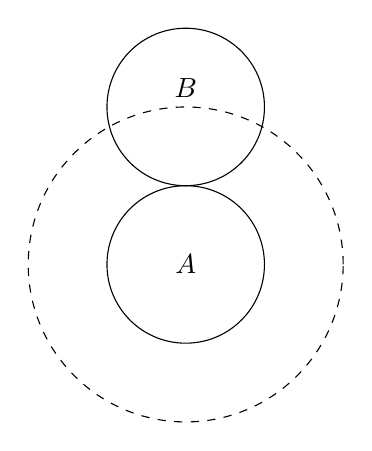
\begin{tikzpicture}
            \draw (0, 0) circle (1);
            \draw (0, 2) circle (1);
            \draw[dashed] (0, 0) circle (2);
            \node[above] at (0, 2) {\(B\)};
            \node at (0, 0) {\(A\)};
        \end{tikzpicture}
        \caption{The excluded volume of one molecule}
        \label{fig:excluded volume}
    \end{figure}
    Figure \ref{fig:excluded volume} shows the excluded volume of molecule \(A\) as the dashed line.
    The excluded region is everywhere that molecule \(A\) makes it impossible for the centre of a molecule to be.
    Molecule \(B\) is as close to molecule \(A\) as possible.
    The exclusion region of a molecule of diameter \(d\) is a sphere of diameter \(2d\).
    The molecular volume is
    \[v = \frac{4}{3}\pi\left(\frac{d}{2}\right)^3\]
    The volume of the exclusion region is
    \[\frac{4}{3}\pi d^3 = 8v\]
    This is shared between two molecules as the exclusion regions can overlap.
    This gives an excluded volume per molecule of \(4v\).
    This gives a molar excluded volume of
    \[b = 4N_Av\]
    The \(a/V_m^2\) term originates from the potential energy.
    Each pairwise interaction lowers the internal energy by \(\epsilon\).
    The number of pairwise interactions for each molecule is proportional to the number of moles divided by the volume, \(n_m/V\).
    The potential energy changes the internal energy of \(n_m\) moles by
    \[U_{PE} = an_m\frac{n_m}{V}\]
    The internal energy change due to changing the volume of the container is
    \[\dd U_{PE} = -\frac{an_m^2}{V^2}\dd V\]
    We associate this with the effective pressure, \(p_\text{eff}\).
    The actual pressure is
    \[p = p_\text{eff} + p_\text{ideal} = p_\text{eff} + \frac{RT}{V_m}\]
    The last one is for one mole of gas.
    Rearranging we get
    \[\frac{RT}{V_m} = p - p_\text{eff} = p + \frac{a}{V_m^2}\]
    since \(n_m = \SI{1}{mol}\).
    We then adjust the volume \(V_m\to V_m - b\) to take account of the excluded volume and we get
    \[\left(p + \frac{a}{V_m^2}\right)(V_m - b) = RT\]
    We only account for the excluded volume in the first order term as the difference is negligible for the second order term.
    
    \subsection{Van der Waal's instability}
    \begin{figure}[ht]
        \centering
        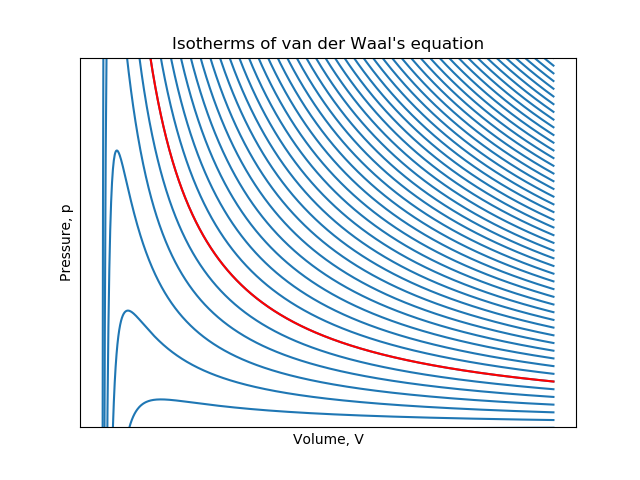
\includegraphics[scale=0.7]{van_der_waals_isotherms.png}
        \caption{Isotherms (lines of constant temperature) of van der Waal's equation.
            The isotherm in red is the critical isotherm at the critical temperature.}
        \label{fig:isotherms of van der Waal}
    \end{figure}
    Figure \ref{fig:isotherms of van der Waal} shows the isotherms (lines of constant temperature) of van der Waal's equation.
    Shown in red is the critical isotherm where the temperature is the critical temperature.
    Van der Waal's equation is only valid for temperatures above the critical temperature.
    The reason for this can be seen in the lower temperature isotherms which behave weirdly at lower volumes and also start to increase slightly at higher volumes when they should asymptote zero.
    
    The isothermal compressibility is less than zero for the isotherms a temperature less than the critical temperature.
    This is because the isothermal compressibility is defined as.
    \[B = -\frac{1}{V}\pdvconst{V}{p}{T}\]
    This should always be positive.
    
    \subsection{Maxwell's Construction}
    What we actually see experimentally is a horizontal line where condensation happens allowing compression without a pressure increase.
    Over the region where this happens liquid and vapour phases are in equilibrium.
    This means that the Gibbs free energy \(\Delta G = 0\).
    Recall that
    \[\dd G = -S\dd T + V\dd p\]
    We define two points \(B_1\) and \(B_2\) which are the edge points of the region where van der Waal's equation predicts that the compressibility is negative.
    We integrate along the isotherm between these two points.
    We get
    \[G(p_{B_1}, T) = G(p_{B_2}, T) + \int_{B_1}^{B_2}V\,\dd p\]
    since temperature is constant so \(\dd T = 0\).
    For \(\Delta G\) to be zero we require
    \[\int_{B_1}^{B_2}V\,\dd p = 0\]
    This means that the area above the isotherm and below the line connecting \(B_1\) and \(B_2\) must be the same as the area below the isotherm and above that line.
    This can in turn be used to find \(B_1\) and \(B_2\).
    
    For temperatures \(T < T_c\) the calculated isotherms from van der Waal's equation oscillate and each passes through a minimum and then a maximum.
    These extrema converge as \(T\to T_c\) and coincide at \(T = T_c\) (ie a point of inflection).
    We can find this from van der Waal's equation:
    \[p = \frac{RT}{V - b} - \frac{a}{V^2}\]
    \[\pdvconst{p}{V}{T} = -\frac{RT}{(V - b)^2} + \frac{2a}{V^3} = 0\]
    \[\pdvconst[2]{p}{V}{T} = \frac{2RT}{(V - b)^3} - \frac{6a}{V^4} = 0\]
    \[RT = \frac{2a(V - b)^2}{V^3} = \frac{3a(V - b)^3}{V^4}\]
    \[\frac{3(V- b)}{V} = 2\]
    This is true only at the critical volume \(V_c\).
    We can substitute this into the second derivative to get
    \[T_c = \frac{8a}{27Rb}\]
    Substituting \(T_c\) and \(V_c\) into van der Waal's equation we get the critical pressure
    \[p_c = \frac{a}{27b^2}\]
    At temperatures \(T < T_c\) how much liquid is present depends on how far along the coexistence region \(V\) is.
    The fraction of the sample that is vapour is given by
    \[f_\text{vap} = \frac{V - V_\text{liq}}{V_\text{vap} - V_\text{liq}}\]
    This is known as Lever's rule.
    As the temperature increases \(f_\text{vap}\) increases and \(V\) is a constant.
    If the number of moles of vapour increases the density of the vapour increases.
    At the critical temperature the point of inflection in \(p\) means that
    \[B = -\frac{1}{V}\pdvconst{V}{p}{T}\to\infty\]
    The compressibility diverges.
    This means that there are large fluctuations in the density.
    This gives rise to critical opalescence where these fluctuations in density cause light to be bounced around a lot and the fluid becomes opaque.
    
    \section{Liquids}
    We can estimate the critical temperature, \(T_c\), using equipartition.
    We know that
    \[\expected{E_K} = \frac{3}{2}k_BT\]
    At the critical point the kinetic and potential energies sum to zero.
    The potential energy is \(-\epsilon\).
    Hence
    \[\frac{3}{2}k_BT_c \approx \epsilon\]
    Often prefactors are dropped in approximations like this giving
    \[T_c \approx \frac{\epsilon}{k_B}\]
    
    \subsection{Lennard--Jones Potential}
    The Lennard--Jones potential is a mathematical model for the potential shown in figure \ref{fig:potential graph}.
    It gives the potential between two particular molecules
    It is a function of distance, \(r\), between the molecules.
    If there are more than two molecules then the total potential due to intermolecular forces is just the sum of the individual potentials between each pair.
    The Lennard--Jones potential is
    \[U_{LJ}(r) = 4\epsilon\left[\left(\frac{\sigma}{r}\right)^{12} - \left(\frac{\sigma}{r}\right)^6\right]\]
    where \(\sigma\) is a constant.
    The \(r^{-12}\) term represents the close range repulsive nature of the potential.
    The \(r^{-6}\) term represents attraction at larger distances.
    Both terms go to zero at infinity as one would expect.
    Compare this to the hard ball model potential where at the molecular diameter the repulsion is infinite and elsewhere it is zero.
    This is basically the same as the Lennard--Jones model but with only two values allowed.
    The Lennard--Jones potential is a bit like having slightly squashable balls instead of hard ones.
    
    The \(r^{-6}\) long range attractive term comes from the attractive van der Waal's interaction:
    \[U(r) = -\frac{C}{r^6} = -\frac{C_\text{dipole} + C_\text{inuction} + C_\text{Dispersion}}{r^6}\]
    The first term comes from the average potential of the dipoles as shown in figure \ref{fig:dipoles}.
    This term is
    \[\expected{U} = -\frac{2}{3k_BT}\frac{\mu_1^2\mu_2^2}{(4\pi\varepsilon_0)^2r^6} = - \frac{C_\text{dipole}}{r^6}\]
    where \(\mu_1\) and \(\mu_2\) are the dipole moments of the two dipoles.
    There are two dipoles so the normal factor of \(r^{-3}\) is squared.
    This term is temperature dependent as the temperature effects how easy it is to move to a more favourable condition.
    \begin{figure}[ht]
        \centering
        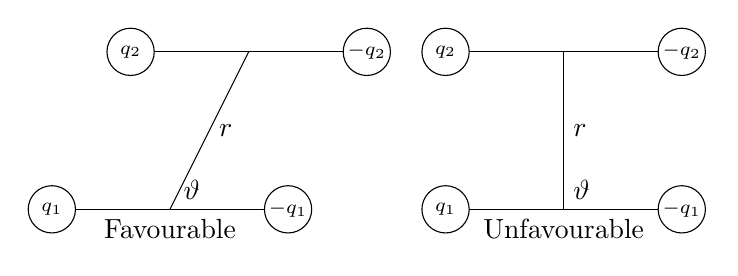
\begin{tikzpicture}
            \draw (0, 0) circle (0.3);
            \node at (0, 0) {\scriptsize\(q_1\)};
            \draw (3, 0) circle (0.3);
            \node at (3, 0) {\scriptsize\(-q_1\)};
            \draw (0.3, 0) -- (2.7, 0);
            
            \begin{scope}[xshift=1cm]
                \draw (0, 2) circle (0.3);
                \node at (0, 2) {\scriptsize\(q_2\)};
                \draw (3, 2) circle (0.3);
                \node at (3, 2) {\scriptsize\(-q_2\)};
                \draw (0.3, 2) -- (2.7, 2);
            \end{scope}
            
            \draw (1.5, 0) -- (2.5, 2);
            \node[right] at (2, 1) {\(r\)};
            \node[above right] at (1.55, 0) {\(\vartheta\)};
            
            \node[below] at (1.5, 0) {Favourable};
            
            \begin{scope}[xshift=5cm]
                \draw (0, 0) circle (0.3);
                \draw (3, 0) circle (0.3);
                \draw (0, 2) circle (0.3);
                \draw (3, 2) circle (0.3);
                \node at (0, 0) {\scriptsize\(q_1\)};
                \node at (3, 0) {\scriptsize\(-q_1\)};
                \node at (0, 2) {\scriptsize\(q_2\)};
                \node at (3, 2) {\scriptsize\(-q_2\)};
                \draw (0.3, 0) -- (2.7, 0);
                \draw (0.3, 2) -- (2.7, 2);
                \draw (1.5, 0) -- (1.5, 2);
                \node[right] at (1.5, 1) {\(r\)};
                \node[above right] at (1.5, 0) {\(\vartheta\)};
                \node[below] at (1.5, 0) {Unfavourable};
            \end{scope}
        \end{tikzpicture}
        \caption{Two dipoles in a favourable and unfavourable configuration}
        \label{fig:dipoles}
    \end{figure}
    The second term appears because of induced dipoles from pre-existing dipoles like in figure \ref{fig:induced dipole}.
    This term is
    \[U_\text{ind}(r) = -\frac{\mu_1^2\alpha_2}{(4\pi\varepsilon_0)^2r^6} = - \frac{C_\text{induction}}{r^6}\]
    where \(\mu_1\) is the dipole moment of the dipole and \(\alpha_2\) is a measure of the strength of the induced dipole.
    The strength of the dipole and the induced dipole both depend on \(r^{-3}\) which explains the factor of \(r^{-6}\).
    \begin{figure}[ht]
        \centering
        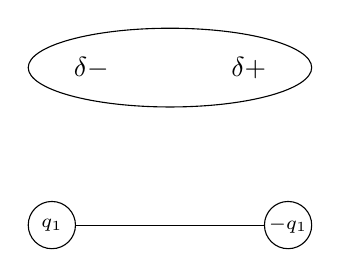
\begin{tikzpicture}
            \draw (0, 0) circle (0.3);
            \node at (0, 0) {\scriptsize\(q_1\)};
            \draw (3, 0) circle (0.3);
            \node at (3, 0) {\scriptsize\(-q_1\)};
            \draw (0.3, 0) -- (2.7, 0);
            \draw (1.5, 2) ellipse (1.8 and 0.5);
            \node at (0.5, 2) {\(\delta{-}\)};
            \node at (2.5, 2) {\(\delta{+}\)};
        \end{tikzpicture}
        \caption{Induced dipole}
        \label{fig:induced dipole}
    \end{figure}
    The third term comes from the different ways that electron spins and can line up and is given by
    \[U_\text{disp}(r) = -\frac{3}{4}\frac{\alpha_0^2I}{(4\pi\varepsilon_r\varepsilon_0)^2r^6} = -\frac{C_\text{dispersion}}{r^6}\]
    
    \subsection{Basic Liquid Properties}
    Liquids exist between the triple and critical points.
    There is a steep gradient on a pressure--volume diagram for a liquid.
    This gives rise to a low compressibility:
    \[B = -\frac{1}{V}\pdvconst{V}{p}{T}\]
    There is typically a \SIrange{10}{15}{\%} increase in volume on melting.
    This is not the case for water or silicon because of their tight packing crystal structures as solids.
    Liquids can't withstand a shear stress.
    The balance between kinetic and potential energy makes theoretical treatment of liquids challenging.
    We will treat liquids as a dense gas (ie the molecular separation is approximately the molecular diameter).
    Liquids have a lower entropy per molecule than a gas.
    This is because there is \emph{some} molecular level order to a liquid.
    
    \subsection{Radial Distribution Function}
    A radial distribution function is a measure of how many molecules there are at a certain distance from a particular molecule.
    To construct it we start by picking an arbitrary test molecule.
    \begin{figure}[ht]
        \centering
        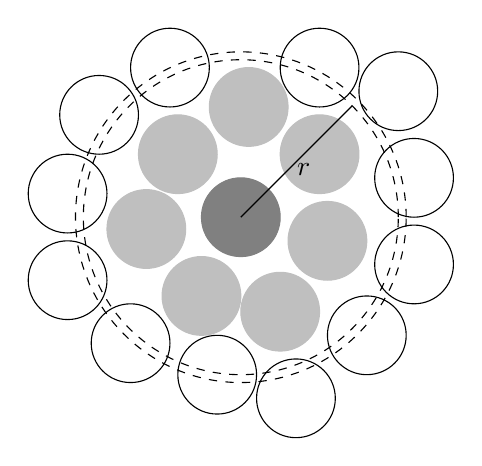
\begin{tikzpicture}
            \draw[color=gray, fill=gray] (0, 0) circle (0.5);
            \draw[color=lightgray, fill=lightgray] (1, 0.8) circle (0.5);
            \draw[color=lightgray, fill=lightgray] (-0.8, 0.8) circle (0.5);
            \draw[color=lightgray, fill=lightgray] (1.1, -0.3) circle (0.5);
            \draw[color=lightgray, fill=lightgray] (0.5, -1.2) circle (0.5);
            \draw[color=lightgray, fill=lightgray] (-0.5, -1) circle (0.5);
            \draw[color=lightgray, fill=lightgray] (-1.2, -0.15) circle (0.5);
            \draw (2, 1.6) circle (0.5);
            \draw (2.2, 0.5) circle (0.5);
            \draw (2.2, -0.6) circle (0.5);
            \draw (1.6, -1.5) circle (0.5);
            \draw (0.7, -2.3) circle (0.5);
            \draw (-0.3, -2) circle (0.5);
            \draw (-1.4, -1.6) circle (0.5);
            \draw (1, 1.9) circle (0.5);
            \draw[color=lightgray, fill=lightgray] (0.1, 1.4) circle (0.5);
            \draw (-0.9, 1.9) circle (0.5);
            \draw (-1.8, 1.3) circle (0.5);
            \draw (-2.2, 0.3) circle (0.5);
            \draw (-2.2, -0.8) circle (0.5);
            \draw[dashed] (0, 0) circle (2);
            \draw[dashed] (0, 0) circle (2.1);
            \draw (0, 0) -- (1.41, 1.41);
            \node at (0.8, 0.6) {\(r\)};
        \end{tikzpicture}
        \caption{Test molecule and spherical shell}
        \label{fig:radial distribution function}
    \end{figure}
    Around this test molecule we construct a spherical shell of radius \(r\) and thickness \(\dd r\).
    The volume of this shell is
    \[\frac{4}{3}\pi ((r + \dd r)^3 - r^3) = \frac{4}{3}\pi(r^3 + 3r^2\dd r + 3r\dd r^2 + \dd r^3 - r^3) = 4\pi r^2\dd r\]
    Where we have disregarded any second order or higher \(\dd r\) terms.
    We define the radially averaged number density function, \(\rho\), as a function of \(r\) such that for a spherical shell of radius \(r\) the number, \(N\), of molecules that intersect the shell is
    \[N(r) = \rho(r)4\pi r^2\dd r\]
    That is \(\rho(r)\) gives the number of molecules per unit volume at a distance \(r\) from the test molecule.
    We then define \(\expected\rho\)\footnote{In the notes this is denoted \(\rho\) but this is confusing as \(\rho\) is already a function so I've decided on a different notation.} as the average number density over the whole sample.
    The radial distribution function, \(g\), is then
    \[g(r) = \frac{\rho(r)}{\expected\rho}\]
    This means that the number of molecules intersecting the spherical shell of radius \(r\) is
    \[N(r) = g(r)\expected\rho 4\pi r^2\dd r\]
    \(N\) can be measured with x-ray or neutron scattering.
    Due to the finite size of the molecules \(\rho(r) = 0\) for \(r < d\) the molecular diameter since we don't count the test molecule and no molecules can be inside the test molecule.
    There is then a spike at about \(d\) where there is a ring of molecules.
    There is then another dip and a smaller spike at \(2d\).
    This is because of the local structure where molecules tend to form spherical shells known as coordination shells.
    At larger distances the number of molecules in the shell tends to a constant amount as there is only local structure in a liquid so \(g(r)\to 1\).
    \begin{figure}[ht]
        \centering
        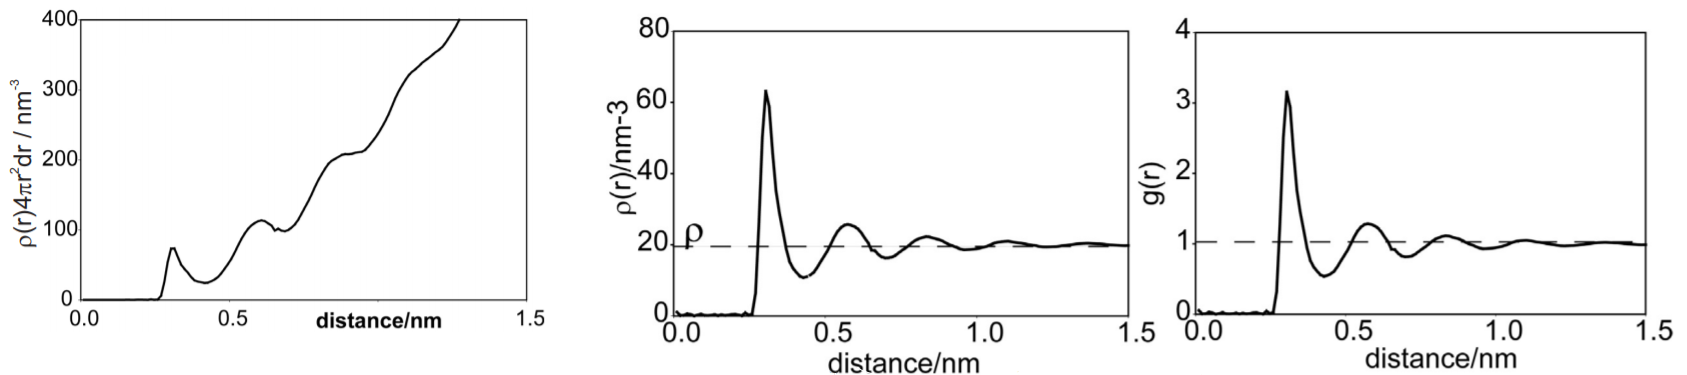
\includegraphics[scale=0.3]{n_rho_g_distribution_functions_plots.png}
        \caption{\(N\), \(\rho\) and \(g\) for argon}
    \end{figure}
    \begin{figure}[ht]
        \centering
        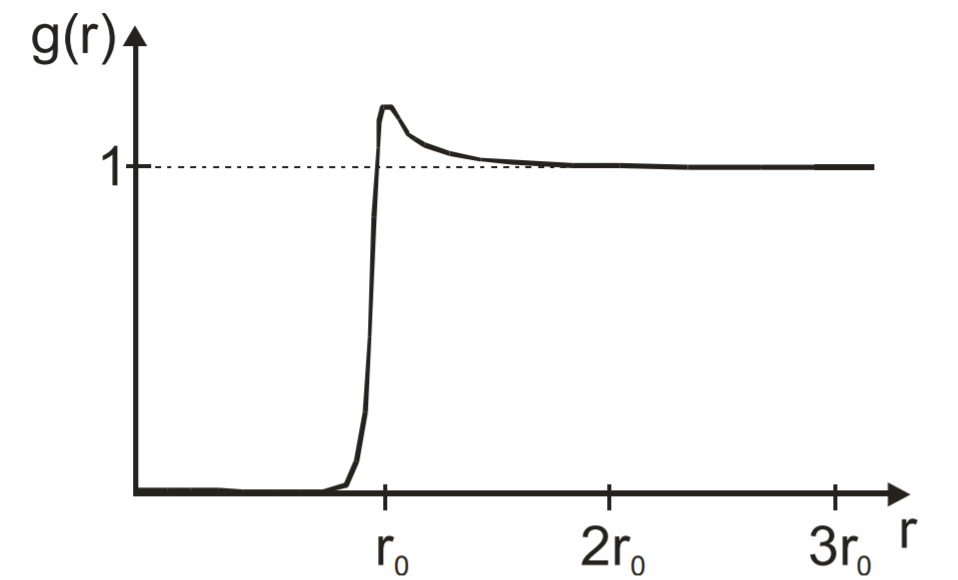
\includegraphics[scale=0.3]{g_distribution_for_gas.png}
        \caption{\(g\) for a real gas}
    \end{figure}
    For an ideal gas we would expect that \(g\) is zero for \(r < d\) and constant for \(r > d\).
    For a real gas we actually see a peak as there is still some local structure but it very quickly tends to a constant.
    
    We define the number of nearest neighbours (also known as the coordination number) as
    \[\int_0^BN(r)\,\dd r = \int_0^B\expected\rho g(r)4\pi r^2\,\dd r\]
    where \(B\) is the distance at which the first trough appears.
    The coordination number is the area under the first peak and is a measure of how many molecules are in the first coordination shell.
    The interaction energy of the test particle with all other molecules is
    \[U' = \int_0^\infty u(r)N(r)\,\dd r = \int_0^\infty u(r)\expected\rho g(r)4\pi r^2\,\dd r\]
    where \(u(r)\) is the pair potential for example Lennard--Jones or the hard sphere potential.
    
    \subsection{Interfacial Properties}
    The surface area to volume ratio for a sphere of radius \(r\) is
    \[\frac{4\pi r^2}{4\pi r^3/3} = \frac{3}{r}\]
    This shows that interfaces are important when objects are small (as in measured in \si{\micro m} or \si{\nano m}).
    The surface free energy, \(\gamma\), is also the surface tension and is the energy cost to create \(\SI{1}{m^2}\) of surface.
    The units are \(\si{J.m^{-2}} = \si{N.m^{-1}}\).
    The reason that it takes energy to create surfaces is that in the bulk of the material the potential is lowered by intermolecular interactions.
    To move a molecule to the surface or remove a layer of molecules to expose a molecule reduces the number of nearest neighbours which increases the potential so work must be done to do this.
    
    In the bulk each molecule has \(N_{nn}\) nearest neighbours and each nearest neighbour reduces the energy by \(\epsilon\).
    At the surface the number of nearest neighbours is reduced by \(\Delta N_{nn}\).
    Therefore there is a higher energy than a molecule in the bulk by \(\epsilon\Delta N_{nn}\).
    The number of molecules in an area \(A\) is given by \(A/r_0^2\)
    where \(r_0\) is the side length of the largest cube that can be constructed around a molecule without including other molecules.
    That is the square with sides \(r_0\) is the area per molecule.
    
    Imagine a column of liquid cut in half to create two surfaces of area \(A\).
    The total new surface area is \(2A\).
    The total free energy cost to do this is the number of molecules now at the surface times the energy increase due to loss of nearest neighbours.
    That is
    \[\epsilon \frac{A}{r_0^2}\Delta N_{nn}\]
    The total free surface energy is the amount \(\gamma\) such that the area created times \(\gamma\) is the energy used to create the surface:
    \[2\gamma A = \epsilon\frac{A}{r_0^2}\Delta N_{nn}\]
    \[\gamma = \frac{1}{2}\frac{\epsilon}{r_0^2}\Delta N_{nn}\]
    
    We can use this to approximate the latent heat of vaporisation.
    Supplying energy \(\epsilon\) separates two molecules.
    To become a vapour a molecule needs to be separated from all of its nearest neighbours so \(\Delta N_{nn} = N_{nn}\).
    The energy needed to transfer one molecule to the vapour phase is \(\epsilon N_{nn}\).
    The energy needed to transfer one mole of molecules to the vapour phase is 
    \[L_\text{vap} = \frac{1}{2}\epsilon N_{nn}N_A\]
    The factor of \(1/2\) accounts for the fact that each pair potential needs breaking only once not once per molecule involved.
    
    We can approximate \(r_0^3\)  as the volume per molecule giving
    \[r_0 = \left(\frac{V}{N}\right)^{\frac{1}{3}}\]
    where \(V\) is the volume and \(N\) is the number of molecules.
    For a liquid with van der Waal's forces \(N_{nn} = 12\) this is the most spheres that can touch one sphere all at the same time, known as the kissing number.
    
    Up to now we have considered the surface free energy.
    We will now show that this is the same as the surface tension.
    consider a rectangle of width \(L\) and initial length \(L\).
    Applying a force, \(F\), along the length increases it by \(\dd x\).
    Increasing the length by \(\dd x\) increases the area by \(\dd A = L\dd x\).
    The work done is \(\gamma\dd A = \gamma L \dd x = F\dd x\) so \(\gamma = F/L\).
    This is a tension and is in fact the surface tension.
    
    For simple liquids \(\gamma\sim \SIrange[range-phrase=-]{30}{100}{\milli J.m^{-2}}\).
    
    \section{Wetting Surfaces and Bernoulli}
    A liquid resting on a solid can do one on the following:
    \begin{itemize}
        \item Wet the surface.
        Wetting occurs when the liquid forms a film over the surface.
        The contact angle \(\vartheta = 0\).
        \item Partially wet the surface.
        Partial wetting occurs when the liquid forms a hemisphere or similar on the surface.
        The contact angle \(\vartheta\in(0, \pi/2)\).
        \item Non-wetting occurs when the liquid forms a bead on the surface.
        The contact angle \(\vartheta > \pi/2\).
    \end{itemize}
    Liquids with low surface free energy wet most solids as the liquid easily spreads out to create a large interfacial area.
    Liquids with high surface free energies in comparison have a non zero contact angle.
    The liquid--liquid interactions are preferable over the liquid--solid interactions and the surface tension acts to keep the liquid together rather than spreading out.
    
    \subsection{Young's Equation}
    The three phase contact line is the line where the solid, liquid and gas are in contact.
    It occurs around the base of a droplet on a solid surface.
    The surface free energy depends on the two materials at the phase boundary.
    To increase the area of solid wetted by \(\dd A\) the surface energy of the solid--liquid interface increases by \(\gamma_{SL}\dd A\).
    Like wise the surface energy of the solid--vapour interface decreases by \(\gamma_{SV}\dd A\).
    Both of these are due simply to the increase in area of the surface--liquid boundary and the necessary decrease in area of the solid--vapour boundary that is replaced by solid--liquid boundary.
    Less obviously the area of liquid--vapour boundary increases by \(\dd A\cos\vartheta\) so the surface energy increases by \(\gamma_{LV}\dd A\cos\vartheta\).
    Conserving energy we get
    \[\gamma_{SV} = \gamma_{SL} + \gamma_{LV}\cos\vartheta\]
    This is Young's equation.
    We could find the same result by balancing the forces that act due to the surface tension given that the droplet must be at rest.
    
    \subsection{Laplace Pressure}
    Suppose a syringe has a drop of liquid of radius \(r\) hanging off the end.
    The pressure of the liquid in the syringe is \(p_1\).
    The pressure outside the syringe is \(p_2\).
    If the piston moves down a distance \(\dd x\) it does work \(\dd W = F\dd x = (p_1 - p_2)\dd V\)
    where \(\dd V\) is the change in volume of the droplet.
    If the radius of the drop increases by \(\dd r\) then
    \[\dd V = \frac{4}{3}\pi((r + \dd r)^3 - r^3) = \frac{4}{3}\pi (r^3 + 3r^2\dd r + 3r\dd r^2 + \dd r^3 - r^3) \approx 4\pi r^2\dd r\]
    Neglecting \(\dd r\) terms raised to powers greater than 1.
    The surface area increases by
    \[\dd A = 4\pi ((r + \dd r)^2 - r^2) = 4\pi (r^2 + 2r\dd r + \dd r^2 - r^2) \approx 8\pi r\dd r\]
    The increase in surface energy must be equal to the work done:
    \[\dd W = (p_1 - p_2)\dd V = 4\pi r^2\dd r(p_1 - p_2) = \gamma\dd A = 8\pi r\dd r\gamma\]
    \[r(p_1 - p_2) = 2\gamma\]
    \[p_1 - p_2 = \frac{2\gamma}{r}\]
    This is called the Laplace pressure.
    
    We can do something similar for a bubble.
    \(p_0\) is the pressure outside the bubble and \(p_\text{bubble}\) is the pressure in the bubble.
    Since there are two interfaces we get an extra factor of two:
    \[p_\text{bubble} - p_0 = \frac{4\gamma}{r}\]
    
    If a surface isn't spherical then we can identify two principle radii of curvature, \(R_1\) and \(R_2\).
    The Laplace pressure is then
    \[p_1 - p_2 = \gamma\left(\frac{1}{R_1} + \frac{1}{R_2}\right)\]
    In the case of a sphere \(R_1 = R_2 = r\) and this reduces to \(2\gamma/r\) as expected.
    Two parallel plates are a distance \(2R_1\) apart.
    The gap is partially filled with liquid.
    The liquid naturally sits in a u shape extending along the length of the plates.
    The first radius of curvature is perpendicular to the plates and has radius \(R_1\).
    The second radius of curvature is parallel to the plates and has an infinite radius of curvature (ie there is no curvature).
    This gives \(p_1 - p_2 = \gamma/R_1\).
    As the plates become further apart \(R_1\to\infty\) and the surface becomes flatter and flatter.
    Eventually there is no curvature and hence no pressure difference.
    
    \subsection{Capillary Rise}
    Dip a narrow tube of radius \(R\) into a liquid which wets the tube.
    This means that the contact angle \(\vartheta = 0\).
    This must be true all around the tube so a cross section along the tube will have a U shaped liquid--vapour interface.
    This is known as a meniscus.
    The radius of curvature of the meniscus will be \(R\).
    The Laplace pressure will be
    \[p_A - p_B = \frac{2\gamma}{R}\]
    where \(p_A\) is the pressure in the tube above the liquid and \(p_B\) is the pressure in the tube in the liquid.
    The pressure \(p_{A'}\) outside of the tube and liquid at the same height as \(p_A\) was measured must be equal to \(p_A\) and approximately equal to the pressure just above the surface of the liquid and all of these must be approximately atmospheric pressure.
    \[p_C - p_B = h\rho g\]
    where \(h\) is the height the liquid is drawn up the tube (to the bottom of the meniscus) and \(\rho\) is the density of the liquid.
    Since \(p_C = p_A\) we can say
    \[p_C - p_B = p_A - p_B \implies \frac{2\gamma}{R} = h\rho g\]
    If instead \(\vartheta\ne 0\) then the radius of curvature is \(R/\cos\vartheta\).
    Balancing the pressure differences again we get
    \[h\rho g = \frac{2\gamma\cos\vartheta}{R}\]
    This even holds for \(\vartheta > \SI{90}{\SIUnitSymbolDegree}\).
    For example mercury \(\vartheta = \SI{140}{\SIUnitSymbolDegree}\) so \(\cos\vartheta < 0\).
    This agrees with what we see which is that the mercury is actually pushed down by the tube rather than being drawn up.
    
    \subsection{Surfactants}
    Water has a high surface tension of \(\gamma = \SI{72}{N.m^{-1}}\).
    Surfactants are molecules that absorb at interfaces lowering the surface tension.
    For example in our lungs there are surfactants in the alveoli.
    Normally \(\gamma = \SI{50}{N.m^{-1}}\) and \(R \sim \SI{e-4}{m}\).
    The required pressure difference to inflate the lungs against surface tension is then \(p_1 - p_2 = 2\gamma/R = \SI{500}{Pa}\).
    This is very big.
    With surfactants \(\gamma = \SI{3}{N.m^{-1}}\).
    This reduces the required pressure difference to \(\SI{30}{Pa}\).
    This is much more manageable.
    
    Alcohol is a surfactant for water.
    This gives rise to the Marangoni effect where wine near the edge of the glass is drawn upwards in the meniscus and due to the increased surface area more alcohol evaporates from this part of the wine so the surface tension increases pulling the wine upwards leading to ``tears" on the wine glass.
    
    \subsection{Fluid Dynamics} 
    Motion of real fluids is very complicated.
    We simplify it by considering two schema:
    \begin{itemize}
        \item Only steady flow with no viscous forces (high Reynold's numbers)
        \item Only steady flow with no inertial forces (low Reynold's numbers)
    \end{itemize}
    We will simplify further by only considering ideal fluids.
    An ideal fluid will in static conditions only undergo steady flow, that is the velocity at a point is constant, ie there is no acceleration at a point (there is still acceleration between points).
    It is also incompressible, that is the density, \(\rho\) is constant.
    The fluid is also non--viscous so there are no viscous losses of energy.
    The flow is irrotational.
    These properties are necessary for us to be able to use conservation of mass and energy.
    
    A streamline is the trajectory followed by a tracer particle.
    It is the path taken by a fluid element.
    Streamlines can't intersect as the velocity is tangent to the streamline so if two intersected it would imply that a fluid element had two different velocities.
    In steady flow streamlines don't move.
    A stream tube is an imaginary tube with stream lines at the boundary.
    Since streamlines can't intersect all fluid in a stream tube remains in the stream tube.
    
    \subsection{Continuity Equation}
    If we apply conservation of mass we get the continuity equation.
    The cross sectional area of a stream tube has the values \(A_1\) and \(A_2\) at two points.
    The velocity at these two points is \(v_1\) and \(v_2\) respectively.
    The volume of fluid through one of these surfaces in time \(\Delta t\) is given by \(v_1A_1\Delta t\) and \(v_2A_2\Delta t\) respectively.
    The mass of fluid through one of these surfaces is then \(\rho_1v_1A_1\Delta t\) and \(\rho_2v_2A_2\Delta t\).
    These values must be the same by conservation of mass.
    Also for an ideal fluid \(\rho_1 = \rho_2\) is constant so
    \[v_1A_1 = v_2A_2\]
    This is the continuity equation.
    For this to hold everywhere along the stream tube we require that in general \(v\propto 1/A\).
    
    \subsection{Bernoulli's Equation}
    Bernoulli's equation is a statement of conservation of energy per unit mass of fluid.
    It only applies if there are no sources or sinks of fluid or energy.
    We start with the same stream tube as from the last section.
    The work done on the system as fluid enters through \(A_1\) is
    \[W_1 = p_1A_1\Delta v_1\Delta t = p_1\frac{\Delta M}{\rho}\]
    since \(p_1A_1\) is the force it imparts and \(\Delta v_1\Delta t\) is the distance it moves the system.
    Likewise the work done on the system as fluid exits through \(A_2\) is
    \[W_2 = p_2A_2\Delta v_2\Delta t = p_2\frac{\Delta M}{\rho}\]
    The net work done is \(W_1 - W_2\) and is the change in energy between 1 and 2.
    \[W_1 - W_2 = p_1\frac{\Delta M}{\rho} - p_2\frac{\Delta M}{\rho} = \frac{1}{2}\Delta Mv_2^2 - \frac{1}{2}\Delta M v_1^2 + \Delta M\varphi_2 - \Delta M\varphi_1\]
    The first two terms account for change in kinetic energy and the second two for change in potential energy. Barring a few weird cases where there is some other potential the potential in question is gravitational and \(\varphi_1 = gh_1\) and \(\varphi_2 = gh_2\) where \(h_1\) and \(h_2\) are the heights of the points 1 and 2 respectively.
    This can be rearranged to give
    \[\frac{p_1}{\rho} + \frac{v_1^2}{2} + \varphi_1 = \frac{p_2}{\rho} + \frac{v_2^2}{2} + \varphi_2 = \text{const}\]
    This is Bernoulli's equation.
    
    \example
    A tank with \(z = 0\) defined as the start height of the water has a hole at \(z = -h\).
    What is the velocity \(v_\text{out}\) at which the water flows out of the tank?
    
    The pressure everywhere is the same and equal to atmospheric pressure.
    The velocity at the top of the tank is zero for a sufficiently large tank.
    The output velocity is \(v_\text{out}\).
    \(\varphi_1 = 0\) and \(\varphi_2 = -gh\).
    This gives
    \[\frac{p_\text{atm}}{\rho} = \frac{p_\text{atm}}{\rho} + \frac{v_\text{out}^2}{2} - gh\]
    \[v_\text{out} = \sqrt{2gh}\]
    This is the same as the velocity of an object that has fallen through a distance \(h\).
    The liquid loses potential energy but gains kinetic energy.
    
    \subsection{Viscosity}
    Viscosity characterises resistance to flow.
    In a viscous fluid kinetic energy is turned into heat.
    Viscosity characterises to what level the shear forces in the fluid are important.
    Consider two planes parallel to each other with a fluid between.
    The top plane moves at a speed, \(v\), relative to the bottom plane.
    This results in a velocity gradient in the fluid.
    The planes exert a shear force on the fluid.
    This shear force is proportional to the shear rate which is the velocity gradient.
    \[\frac{F}{A} = \eta\dv{v}{y}\]
    where \(v\) is the velocity of the fluid, \(F\) is the force moving the top plate and \(A\) is the area of the plates.
    \begin{figure}[ht]
        \centering
        \begin{tikzpicture}
            \draw (0, 0) rectangle (5, -0.25);
            \draw (0, 3) rectangle (5, 3.25);
            \draw[->] (5, 3.125) -- (6, 3.125);
            \node[right] at (6, 3.125) {\(F\)};
            \draw (1.5, 0) -- (1.5, 3);
            \draw (1.5, 0) -- (3.5, 3);
            \node[left] at (0, -0.125) {\(v = 0\)};
            \draw[->] (1.5, 1.5) -- (2.5, 1.5);
            \node[right] at (2.5, 1.5) {\(v(y)\)};
            \draw[->] (-1, 1) -- (-1, 2);
            \node[above] at (-1, 2) {\(y\)};
        \end{tikzpicture}
        \label{Shear force on a fluid}
    \end{figure}
    %%%%%%%%%%%%%%%%%%%%%%%%%%%%%%%%%%%%%%%%%%%%%%%%%%%%%%%%%%%%%%%%%%%%%%%%%%%%%%%%%%%%%%%%%%%%%%%%%%%%%%%%%%%%%%%%%%%%%%%%%%%%%%%%%%%%%%%%%%%%%%Finish end of lecture on fluid mechanics here
    
    \input{Matter_Lecture_Notes_Part_2.tex}
\end{document}
